\documentclass[12pt,final,twoside]{report}
%%%%%%%%%%%%%%%%%%%%%%%%%%%%%%%%%%%%%%%%%%%%%%%%%%%%%%%%%%%%%
% Some credits:
% The template initially was created by Prof. Dr. Holger Karl/Uni Paderborn '2006
% and was expanded and updated by 
% - Stefan Heinrich/Uni Paderborn/Uni Hamburg since 2008,
% - Sven Magg/Uni Hamburg since 2013.
% Suggestions for changes are always welcome.
%%%%%%%%%%%%%%%%%%%%%%%%%%%%%%%%%%%%%%%%%%%%%%%%%%%%%%%%%%%%%
% Meta information:
\newcommand{\trtitle}{Adaptive Learning Strategies for Neural Paraphrase Generation}
\newcommand{\trtype}{Master Thesis} %{Bachelorthesis} %{Diplomarbeit} %{Dissertation}
\newcommand{\trcourseofstudies}{Intelligent Adaptive Systems} %{Bioinformatik} %{Intelligent Adaptive Systems} 
\newcommand{\trauthor}{Ethem Can Karaoguz}
\newcommand{\trauthordegree}{} %{\ B.Sc.}
\newcommand{\tremail}{4karaoguz@informatik.uni-hamburg.de}
\newcommand{\trmatrikelnummer}{6641214}
\newcommand{\trgutachterA}{\href{mailto:beimann@informatik.uni-hamburg.de}{Prof. Dr. Chris Biemann}}
\newcommand{\trgutachterB}{\href{mailto:yimam@informatik.uni-hamburg.de, milde@informatik.uni-hamburg.de}{Seid Muhie Yimam, Benjamin Milde}}
%\newcommand{\trbetreuung}{\href{mailto:tbd@informatik.uni-hamburg.de}{Dipl.-Inform. To Be Defined}}
\newcommand{\trfach}{Language Technology Lab}
\newcommand{\trdate}{22.08.2018}
\newcommand{\trkeywords}{Learning, Language, NLP, Deep Learning}
%Optionally: it is also allowed to provide a street name on the
%\newcommand{\trstrasse}{Streetname 42}
%\newcommand{\trort}{22527 Hamburg}

%%%%%%%%%%%%%%%%%%%%%%%%%%%%%%%%%%%%%%%%%%%%%%%%%%%%%%%%%%%%%
% Languages:

% Falls die Ausarbeitung in Deutsch erfolgt:
% \usepackage[german]{babel}
% \usepackage[T1]{fontenc}
% \usepackage[latin1]{inputenc}
% \usepackage[latin9]{inputenc}                     
% \selectlanguage{german}

% If the thesis is written in English:
\usepackage[english]{babel}                         
\selectlanguage{english}

%%%%%%%%%%%%%%%%%%%%%%%%%%%%%%%%%%%%%%%%%%%%%%%%%%%%%%%%%%%%%
% Bind packages:
\usepackage{acronym}                    % Acronyms
\usepackage{algorithmic}                % Algorithms and Pseudocode
\usepackage{algorithm}                  % Algorithms and Pseudocode
\usepackage{amsfonts}                   % AMS Math Packet (Fonts)
\usepackage{amsmath}                    % AMS Math Packet
\usepackage{amssymb}                    % Additional mathematical symbols
\usepackage{amsthm}
\usepackage{adjustbox}
\usepackage{booktabs}                   % Nicer tables
%\usepackage[font=small,labelfont=bf]{caption} % Numbered captions for figures
\usepackage{color}                      % Enables defining of colours via \definecolor
\definecolor{uhhRed}{RGB}{226,0,26}     % Official Uni Hamburg Red
\definecolor{uhhGrey}{RGB}{136,136,136} % Official Uni Hamburg Grey
\definecolor{uhhLightGrey}{RGB}{220, 220, 220}
\usepackage{fancybox}                   % Put equations in a frame
\usepackage{fancyhdr}                   % Packet for nicer headers
%\usepackage{fancyheadings}             % Nicer numbering of headlines
\usepackage[body={5.8in,9in}]{geometry} % Type area (size, margins...)

%\geometry{a4paper,outer=3.35cm}        % !!!Release version (Normal margins)
%\geometry{a4paper,outer=2.5cm}         % !!!Print version (Additional margin on the left for the binding)
%\geometry{a4paper}                     % !!!Proofread version (Additional margin on the right for corrections)
\geometry{a4paper,outer=3.134cm}        % !!!Draft version (Same margins on left and right)
%\geometry{paperheight=10.0in,paperwidth=6.4in,top=0.51in,left=0.3in}  % !!!Developer version (Minimal margins)

\usepackage{graphicx}                   % Inclusion of graphics
%\usepackage{latexsym}                  % Special symbols
\usepackage{longtable}                  % Allow tables over several parges
\usepackage{listings}                   % Nicer source code listings
\usepackage{multicol}                   % Content of a table over several columns
\usepackage{multirow}                   % Content of a table over several rows
\usepackage{rotating}                   % Alows to rotate text and objects
%\usepackage{siunitx}					% Nicer display of units and number according to SI standards
%\sisetup{tight-spacing=true}  
\usepackage[hang]{subfigure}            % Allows to use multiple (partial) figures in a fig
%HINT: subfigure may be depricated already - maybe try subfig instead 
%\usepackage[font=footnotesize,labelfont=rm]{subfig}    % Pictures in a floating environment
\usepackage{tabularx}                   % Tables with fixed width but variable rows
\usepackage{url,xspace,boxedminipage}   % Accurate display of URLs

%%%%%%%%%%%%%%%%%%%%%%%%%%%%%%%%%%%%%%%%%%%%%%%%%%%%%%%%%%%%%
% PDF Information und Definitions:
\author{\trauthor}

\ifx\pdftexversion\undefined
\usepackage{hyperref}
\else
\usepackage[colorlinks=false,           % link is colores (true) or has colored frame (false)
            linkcolor=uhhRed,           % case colorlinks=true: define color.
            urlcolor=uhhRed,
            citecolor=uhhRed,
            bookmarks,                  % Place bookmarks erstellen
            bookmarksopen=true,         % Bookmarks will be shown at start (true/false)
            pdfpagemode=UseOutlines,    
            bookmarksopenlevel=1,       % Define the depth of shown links
            bookmarksnumbered,          % Numbers of chapers in Bookmarks
            pdftitle={\trtitle},
            pdfsubject={\trtype},
            pdfkeywords={\trkeywords},
            pdfauthor={\trauthor},
            plainpages=false
            ]{hyperref}
\fi

\ifx\pdftexversion\undefined
\else
\pdfoutput=1                            % Disable PDF-Output
\pdfimageresolution=1200
\pdfcompresslevel=2                     % 0 = no compression, 9 = strongest compression
\fi

%%%%%%%%%%%%%%%%%%%%%%%%%%%%%%%%%%%%%%%%%%%%%%%%%%%%%%%%%%%%%
% Configurationen:

\hyphenation{whe-ther}                  % Manually use: "\-" in a word: Staats\-ver\-trag

%\lstloadlanguages{C}                   % Set the default language for listings
\DeclareGraphicsExtensions{.pdf,.svg,.jpg,.png,.eps} % first try pdf, then eps, png and jpg
\graphicspath{{./src/}}                 % Path to a folder where all pictures are located
\pagestyle{fancy}                       % Use nicer header and footer

% Redefine the environments for floating objects:
\setcounter{topnumber}{3}
\setcounter{bottomnumber}{2}
\setcounter{totalnumber}{4}
\renewcommand{\topfraction}{0.9}        %Standard: 0.7
\renewcommand{\bottomfraction}{0.5}     %Standard: 0.3
\renewcommand{\textfraction}{0.1}       %Standard: 0.2
\renewcommand{\floatpagefraction}{0.8}  %Standard: 0.5

% Tables with a nicer padding:
\renewcommand{\arraystretch}{1.2}

% Chapter and Sections will not be written in capitals
\renewcommand{\chaptermark}[1]{\markboth{\chaptername \ \thechapter.\ #1}{}}
\renewcommand{\sectionmark}[1]{\markright{\thesection.\ #1}}

% Avoid french spacing (double spacing after a full stop)
\frenchspacing

%%%%%%%%%%%%%%%%%%%%%%%%%%%%
% Additional 'theorem' and 'definition' blocks:
\theoremstyle{plain}
\newtheorem{theorem}{Theorem}[chapter]
%\newtheorem{theorem}{Satz}[chapter]    % Wenn in Deutsch geschrieben wird.
\newtheorem{axiom}{Axiom}[chapter]     
%\newtheorem{axiom}{Fakt}[chapter]      % Wenn in Deutsch geschrieben wird.
%Usage:%\begin{axiom}[optional description]%Main part%\end{fakt}

\theoremstyle{definition}
\newtheorem{definition}{Definition}[chapter]

%Additional types of axioms:
\newtheorem{lemma}[axiom]{Lemma}
\newtheorem{observation}[axiom]{Observation}

%Additional types of definitions:
\theoremstyle{remark}
%\newtheorem{remark}[definition]{Bemerkung} % Wenn in Deutsch geschrieben wird.
\newtheorem{remark}[definition]{Remark} 

%%%%%%%%%%%%%%%%%%%%%%%%%%%%
% Provides TODOs within the margin:
\newcommand{\TODO}[1]{\marginpar{\emph{\small{{\bf TODO: } #1}}}}

%%%%%%%%%%%%%%%%%%%%%%%%%%%%
% Abbreviations and mathematical symbols
\newcommand{\modd}{\text{ mod }}
\newcommand{\RS}{\mathbb{R}}
\newcommand{\NS}{\mathbb{N}}
\newcommand{\ZS}{\mathbb{Z}}
\newcommand{\dnormal}{\mathit{N}}
\newcommand{\duniform}{\mathit{U}}

\newcommand{\erdos}{Erd\H{o}s}
\newcommand{\renyi}{-R\'{e}nyi}
% it is recommented to define complex terms as expression/newcommand and use the expression in the tex instead.

%%%%%%%%%%%%%%%%%%%%%%%%%%%%%%%%%%%%%%%%%%%%%%%%%%%%%%%%%%%%%
% Document:

\begin{document}

\pagenumbering{Roman}                   % Roman pagenumbering for lists and meta pages
\renewcommand{\headheight}{14.5pt}      % Size of headings

\thispagestyle{empty}
\fancyhead[LO,RE]{}                     % Define the header style for the meta pages

%%%%%%%%%%%%%%%%%%%%%%%%%%%%
% Cover sheet

\begin{titlepage}
%---Possibility 1:
    \begin{flushleft}
        
\includegraphics[width=67mm, scale =1.5]{uhhLogoL.pdf}\\
    \end{flushleft}
    \rule{\textwidth}{0.4pt}
        \newline
        \vspace{2.0cm}
        \begin{center}
          \LARGE \textbf{\trtitle}
        \end{center}
    \vspace{2.0cm}
    \begin{center}
      \textbf{\trtype}\\
      %im Arbeitsbereich \trfach\\
      at Research Group \trfach\\
      \trgutachterA\medskip\\
      %Fachbereich Informatik\\
      Department of Informatics\\
      %MIN-Fakult\"at\\
      MIN-Faculty\\
      Universit\"at Hamburg \\[1.0cm] %not allowed to translate Universit{\"a}t Hamburg
      %vorgelegt von \\
      submitted by \\
      \textbf{\href{mailto:\tremail}{\trauthor\trauthordegree}}\\
      %Studiengang:   \trcourseofstudies \\
      Course of study:   \trcourseofstudies \\
      Matrikelnr.:  \trmatrikelnummer \\
      %a\\
      on\\
      \trdate
    \end{center}
    \vspace{2cm}
    \begin{center}
    \begin{tabular}{ll}
    %Gutachter: & \trgutachterA \\
    Examiners: & \trgutachterA \\
                   & \trgutachterB \\
    %Betreuung: & \trbetreuung \\    	% Adviser are not allowed to demand getting mentioned here, but are happy getting credited by student's initiative
    \end{tabular}
    \end{center}
    \vfill
%    \begin{tabular}{l}
%    \trauthor \\
%    Matrikelnummer:  \trmatrikelnummer \\
%    \trstrasse \\
%    \trort
%    \end{tabular}
%    \newline
    \rule{\textwidth}{0.4pt}
    \newpage 
\end{titlepage}

    %backsite of cover sheet is empty!
\thispagestyle{empty}
\hspace{1cm}
\newpage

%%%%%%%%%%%%%%%%%%%%%%%%%%%%
% Abstract:
\section*{Abstract}\label{sec:abstract}

Continuously learning from a data stream in NLP applications, is an important challenge for deep neural models. This thesis studies the applicability and the behaviour of deep neural models in a setting where the training data comes from a continuous data stream. We propose adaptive learning strategies for neural paraphrase generation which are based on incremental, transfer and active learning. We simulate a continuous data stream by dividing an existing dataset randomly into subsets and feeding these subsets to the model iteratively. We demonstrate that integration of a deep neural model with a continuous data stream, is possible and practical. Experimental results show that the neural model is able to adapt to the continuous data stream, increasing its' performance through time. Additionally, one of the proposed incremental learning strategies is able to outperform traditional supervised learning, increasing the overall BLEU score by 2.76. Moreover the model is able to learn much faster with incremental learning than traditional supervised learning, former outperforming the latter with only 60 percent of the dataset. We also make an analysis of transfer learning for paraphrase generation, to show if knowledge transfer is possible for paraphrase generation. We conduct experiments in order to determine what aspects of the neural network are actually transferred. Moreover we test four different transfer methods which are designed for specific use cases. The experimental results on transfer learning show that success of the knowledge transfer depends on the context and size of the source and target datasets. We show that when the transfer is successful, both hidden layers and word embeddings are transferred. The results regarding the different transfer methods show that restricting the model on target dataset leads to poor performance especially in incremental setting. Sampling methods we used for active learning are proven to be ineffective on the paraphrase generation task leading no improvements on both overall BLEU score and training data usage. We also show that in a case of concept drift, the model is able to successfully adapt to the new training data despite the fact that it is previously trained on a different dataset.


%\fancyhead[LE,RO]{\it Abstract}
%\addcontentsline{toc}{chapter}{\numberline{}Abstract}
	


%% If the abstract ist not longer than half a page, then the German Zusammenfassung can be places on the same page
%%\cleardoublepage
%\vfill
%\section*{Zusammenfassung}\label{sec:zusammenfassung}
%%\addcontentsline{toc}{chapter}{\numberline{}Zusammenfassung} %Add the Zusammenfassung to the TOC
%Hier die deutsche Zusammenfassung einf\"ugen (notwendig).
%\fancyhead[LE,RO]{\it Abstract}

%\cleardoublepage

%%%%%%%%%%%%%%%%%%%%%%%%%%%%
% Lists:
%\setcounter{tocdepth}{1}               % depth of the table of contents (for BSc and MSc Thesis 1 is recommented)
\fancyhead[LE,RO]{\it Contents}
\tableofcontents
\cleardoublepage
% List of Figures and List of tables are optional. -> Not needed in most theses.
\fancyhead[LE,RO]{\it List of Figures}
\listoffigures
%\cleardoublepage
\fancyhead[LE,RO]{\it List of Tables}
\listoftables
%\cleardoublepage
%\lstlistoflistings
%\cleardoublepage

\fancyhead[LE]{\it \leftmark}           % Define the header style for the text pages
\fancyhead[RO]{\it \rightmark}          % Define the header style for the text pages
\fancyhead[LO,RE]{}                     % Define the header style for the text pages

%%%%%%%%%%%%%%%%%%%%%%%%%%%%
% The content will be included here:
\pagenumbering{arabic}

\chapter{Introduction}\label{introduction}

Generally, machine learning applications build models depending on training data which is gathered collectively by using a specific data acquisition tool. This process introduces a number of problems regardless of quality and amount of the gathered training data. First of all, the data acquisition process itself can cost lots of time and money since the data has to be labelled by human workers. Moreover if the domain in which the training data is collected from is very specific, for example medical text, certain number of domain experts might be needed. In the cases where the domain experts cannot be employed, gathering necessary amount of data to build a model can be impractical or impossible. Secondly, training on previously gathered large datasets with traditional supervised learning can be very computationally expensive. Thirdly and most importantly, data distribution of the domain where the target application operates can change which leads to existing training data to become outdated. Since the model is not trained with the changed data coming from the environment, it performs poorly. This phenomenon is called concept drift in the literature \cite{concept}. In this case more training data has to be gathered and the model has to be re-trained with the new data, both of which can be again impractical or impossible depending on the resources at hand.

These mentioned problems make us to think about a data acquisition process where the training data is collected interactively and iteratively with a model which adapts to the continuous data stream. In the proposed design, the model is trained continuously with each iteration of data acquisition process instead of training by traditional supervised learning with large amount of data. The model not only aims to automatically adapt to new training data without any retraining from scratch, it also interacts with human users by providing suggestions to users and making use of user feedback as a form of input to train. With this human-in-the-loop paradigm, necessity of collecting a large dataset in advance is eliminated and a functional model (even though it is not fully optimal to use) is created very fast, at the same time. This paradigm is called adaptive learning. Figure 1.1 shows the basic workflow of suggested data acquisition process. The goal is to create a model which has comparable or better performance than a model trained with traditional supervised learning at the end of data acquisition process. Figure 1.2 shows a real world human-in-the-loop data acquisition system for text simplification.

\begin{figure}[h]
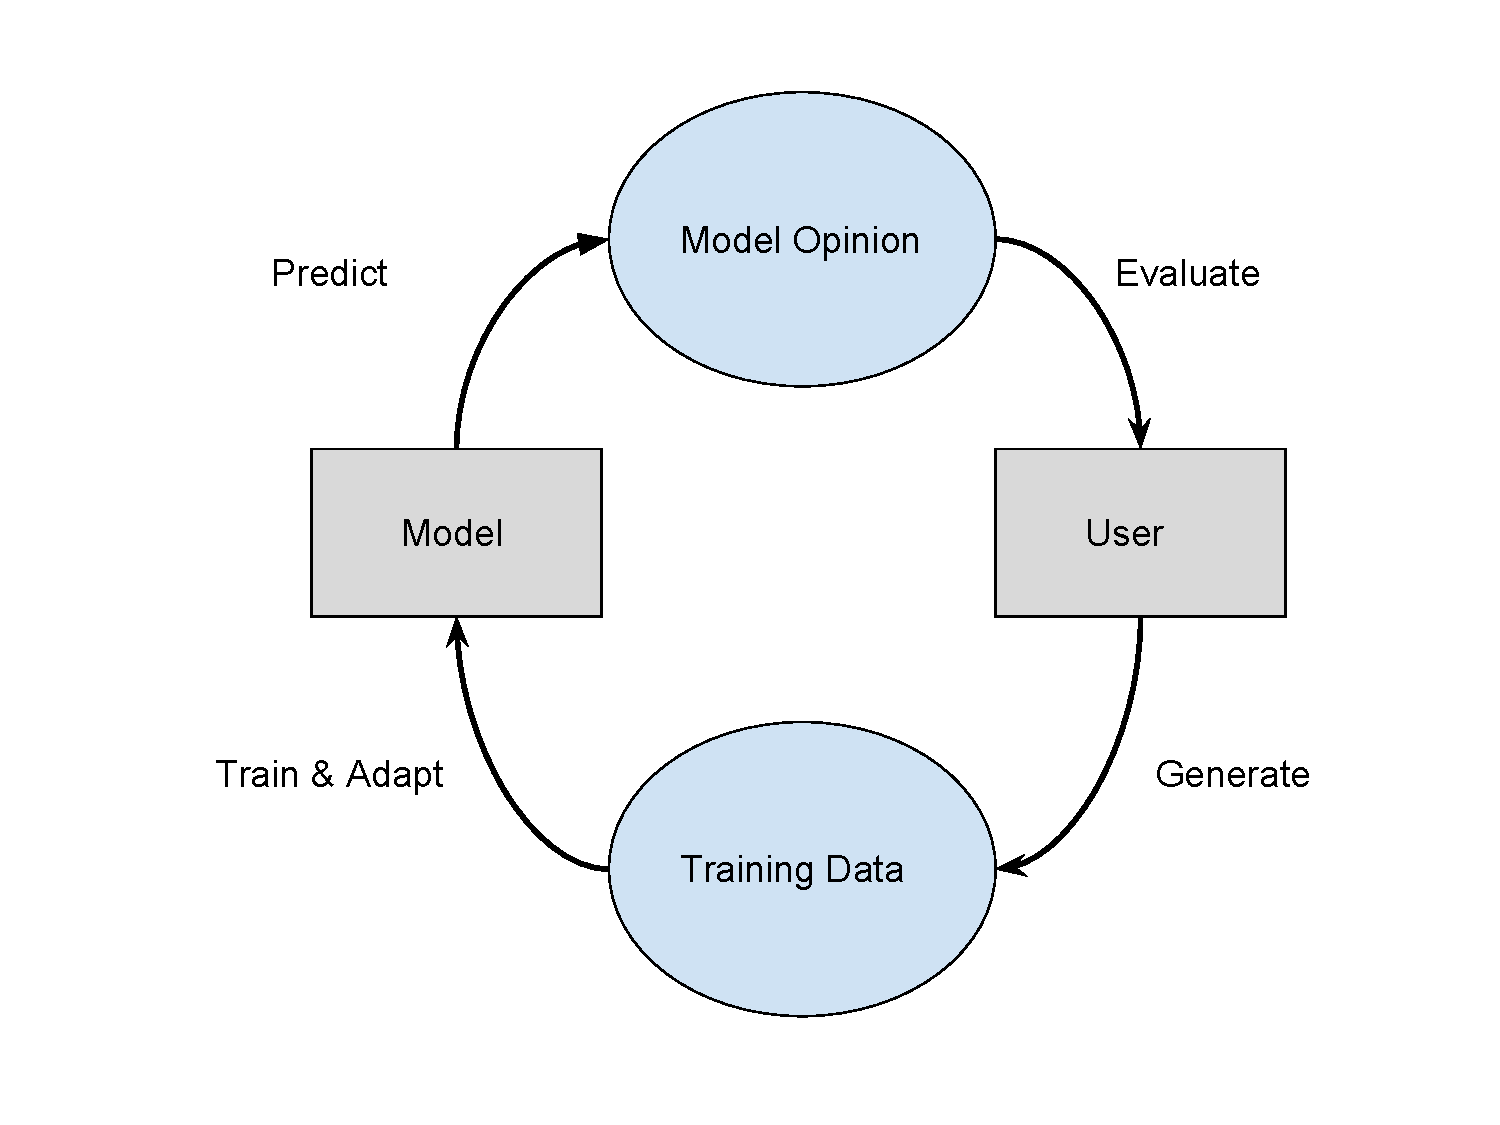
\includegraphics[width=\textwidth, height=10cm]{hil}
\centering
\caption{Human in the loop data acquisition.}
\end{figure}

Main focus of this thesis is the behaviour of deep neural models in human-in-the-loop settings which is described above. Different learning strategies for training deep neural models are studied and experiments with different training methods are conducted in order to investigate their effectiveness in continuous data streams. Additional learning strategies are also proposed in order to overcome some of the problems which are introduced by human-in-the-loop setting. Although human-in-the-loop data acquisition can help with the problems which are described in the beginning of this section, it also introduces some other problems in the context of modelling. As a starting point, it is shown that a deep neural model in fact can adapt and improve with the continuously increasing data and then different learning strategies are studied, each of which addressing a different problem in human-in-the-loop setting. Instead of traditional supervised learning, incremental learning is studied in order to obtain adaptivity to incoming data without forgetting previous knowledge. Learning strategies that are proposed, are mainly concerned with how the model processes the incoming data. 

Incremental learning is shown to be able to create a relatively good and usable model, way before the model is exposed to all of the training data. Experiments with transfer learning are done in order to simulate a concept drift scenario where a general model comes across to new training data with different nature. With the same experiments, a situation in which the system does not have enough resources to collect significant amount of data, is also simulated. It is also shown that with transfer learning, it is possible to create a model which is impossible to create with the available data. Additionally, different active learning strategies are studied in order to reduce the data we need to build a satisfactory model.  At the end, experiments in which these strategies are combined together are done and their results are reported.

\begin{figure}[h]
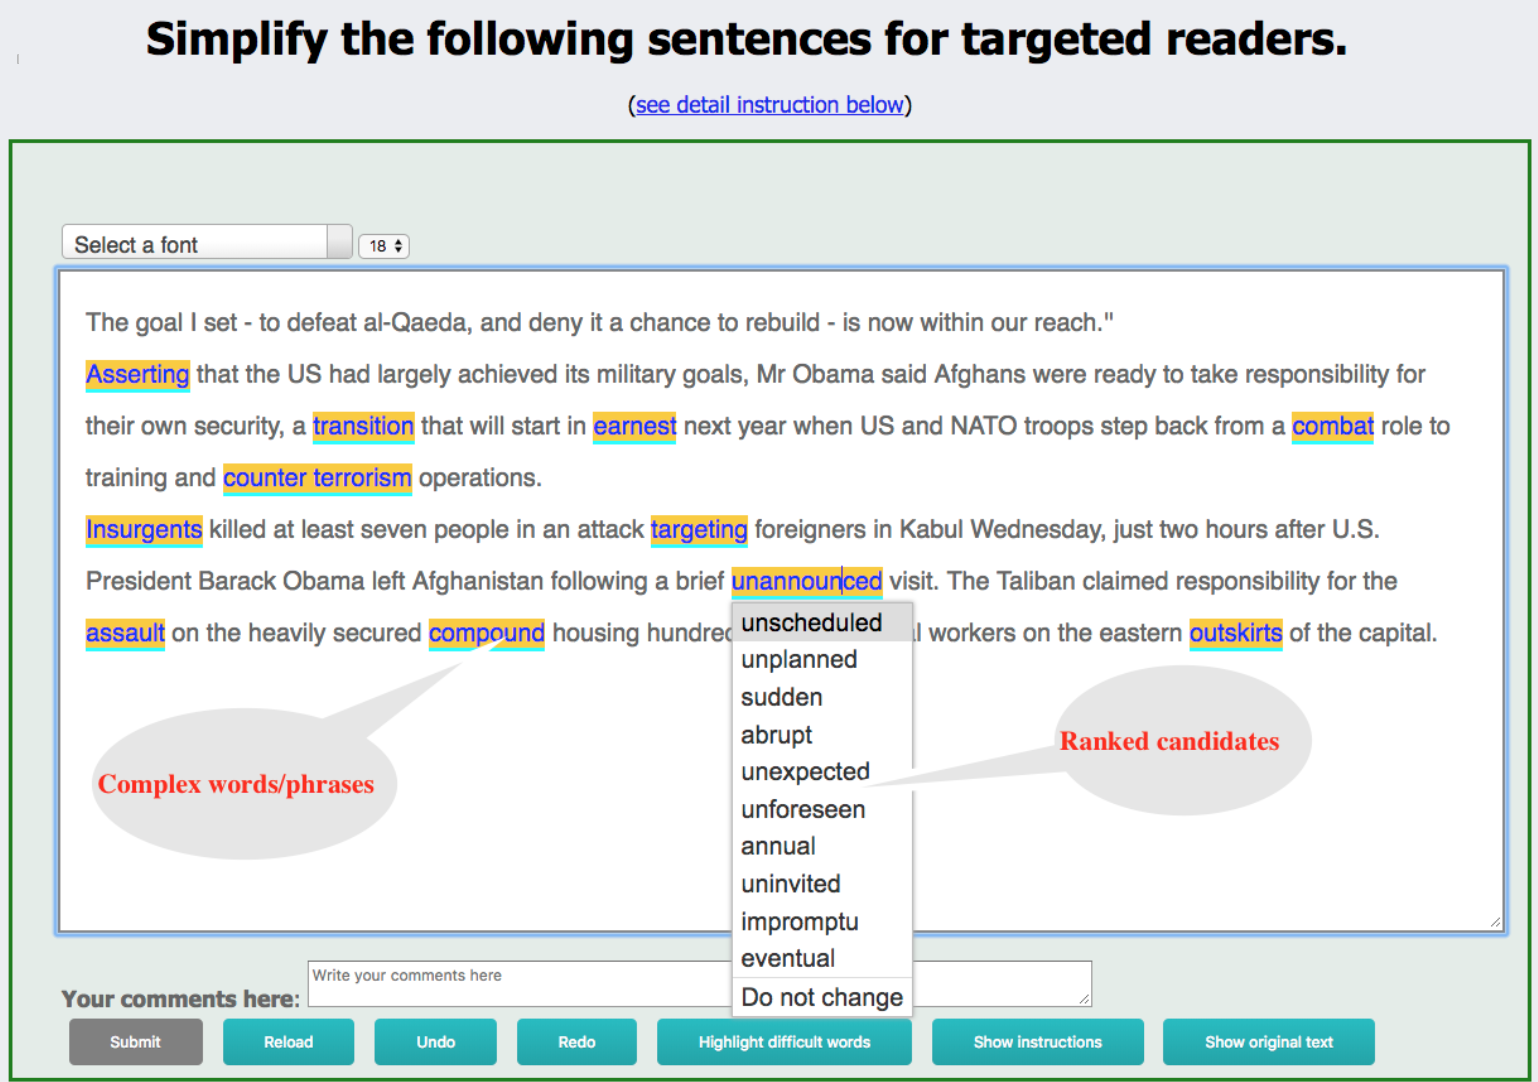
\includegraphics[width=\textwidth]{human-in-the-loop}
\centering
\caption{An interactive human-in-the-loop application for text simplification \cite{par4sim}. Target words to be simplified are highlighted and user is provided with a list of candidate words to choose from. Candidate words are generated and ranked by the system/model.}
\end{figure}


Paraphrase generation is chosen as the target application. Paraphrase generation is the problem of generating different texts from a source text while retaining the meaning. It has various application areas in Natural Language Processing (NLP) like dialogue systems where it is used for building more natural conversional agents, information retrieval where it is used for enhancing retrieval process, natural language generation where it is used for generating training data for different NLP tasks and text summarization where it is used for replacing a text with a simpler paraphrase of it. Generating the text "President Trump strongly denied any wrong doing in this matter." from the text "POTUS firmly denied any fault in this subject." would be a good example of paraphrase generation. It is a challenging problem because of many different reasons. There are more than one way to paraphrase a source sentence and the quality of generated paraphrase depends on many things like context information, lexical and semantic diversity and so on. Therefore the problem is not only concerned with language generation, it also deals with language understanding. Another problem which is introduced by picking paraphrase generation as our target application is out of vocabulary words. 

Deep neural models for NLP problems is built on predefined and specific vocabularies which are usually constructed from training data. These vocabularies cannot be changed or expanded during or after training. Since the model does not know the words which it have not seen in the training, unknown words can lead to poor performance. This is an open problem in NLP and all neural models suffer from it but in our case it is more problematic because of the setting which is studied and nature of the problem. In our setting data comes to the system continuously and the model is trained continuously therefore adapting model strictly depends on the vocabulary which it started training with. Additionally paraphrase generation is not a classification or regression task, it is a generation task therefore we do not know target texts (paraphrases) for our source texts beforehand, they are generated by users. These two mentioned reasons cause our model to be more prone to out of vocabulary words since there will be more of them compared to traditional supervised setting. There are two possible solutions for this problem. First solution is to use pre-trained word embeddings for our neural net instead of training our own word embeddings. These pre-trained word embeddings are built on very large corpuses so they would cover a lot of out of vocabulary words for our training data. Second solution is to design a data acquisition process similar to \cite{par4sim} where the system suggests paraphrase candidates which are created from large, existing resources and make the user choose from suggestions. Even though this puts restrictions to the users, it ensures that the target paraphrases are built from a known vocabulary. Since the vocabulary is known beforehand the model can train its own word embeddings. In this thesis the latter solution is simulated. 

The human-in-the-loop process described in this section is simulated by dividing a large existing dataset into subsets and feed the model with these subsets iteratively. In each iteration, the model gets a new batch of data and updates itself according to it. The model is trained with these batches using different learning strategies and evaluate it on a separate test set at the end of each iteration, observing the model's behaviour through time.

According to our knowledge there is no work studying neural paraphrase generation in human-in-the-loop settings especially concerning adaptivity of the neural model. Moreover this work seems to be first to try incremental learning and active learning for neural paraphrase generation. This thesis also builds on to existing transfer learning research for neural paraphrase generation by experimenting with different methods of transfer and analysing the transfer process.

\section{Thesis Organization}
This thesis is organized as follows; the rest of this chapter provides the research questions that are investigated and a review of state-of-the-art works in neural paraphrase generation, human-in-the-loop learning and the learning strategies used in this work. In Chapter 2, the main methodology and technical details regarding our deep neural model are explained which are followed by the description of main ideas behind the learning strategies. Chapter 3 describes the details of the learning strategies, the datasets and evaluation metric used in this work. It also explains the experimental setups in detail with their corresponding reasonings. In Chapter 4, results of the experiments are presented, the findings are explained and a discussion on the overall findings of the thesis is provided. The two last chapters give the conclusion and an extensive list of future work.

\section{Research Questions}

This thesis is going to aim to investigate whether deep neural models can be combined with adaptive learning, human-in-the-loop paradigm for paraphrase generation task. The basic research questions can be summarized as below:

\begin{itemize}
  \item Can deep neural models effectively adapt and gradually perform in a continuous data stream for paraphrase generation?

Considering the fact the deep neural models need a lot of training data to perform well, is it possible to integrate this type of models into human-in-the-loop setting? The model is expected to learn and adapt continuously since retraining large models over and over again through time, is not desirable. The main goal is to determine whether such models can be applied to real world applications which have similar setting to ours. If the answer is yes, what should be the training scheme (how to make use of incoming data stream) for such models? Basically we would like to know if continuous learning is possible for neural paraphrase generation. 
 
  \item Can the model achieve better or comparable performance than traditional supervised learning by leveraging the data stream?
  
  Can adaptive learning improve accuracy by adding more generalization power? Can the model achieve better or comparable performance with less data? It is also possible that training a deep neural network in adaptive manner may have a negative effect, if so it will be insightful to understand the reason why. Understanding how deep models behave under this training paradigm is an interesting and challenging question.
   
  \item What are the possible challenges/limitations introduced by system and model in this setting and what are the possible learning strategies that can be used for dealing with these challenges?
  
  It is important to determine what kind of existing learning strategies that can used to perform better in human-in-the-loop setting. This is particularly important since the setting itself imposes some challenges. How can the model deal with challenges like limited resources and concept drift? Additionally training deep neural models continuously introduces challenges of its own like overfitting and underfitting depending on the training data.

\end{itemize}

Considering the lack of research in this area, with these questions answered, it might be possible to enhance the performance of deep neural models (shorter training time and / or better paraphrases) in paraphrase generation task and create a framework on adaptive learning for future research.

\section{Related Work}

Deep learning based approaches have been quite successful in various NLP tasks including language modelling \cite{siriam}, automatic speech recognition \cite{hannun} and neural machine translation \cite{cho}. Main idea behind deep learning is learning future representations of the dataset instead of depending on hand crafted features engineered by domain experts. Deep neural models is capable of hidden representations and relationships inside the data which are not possible to obtain by feature engineering. In the case of NLP, deep neural models are capable of capturing lexical, semantical and contextual relationships between textual data points which makes them quite successful. Nowadays, almost all of the state-of-the-art models used in NLP applications are based on deep learning.

For the task of paraphrase generation, deep learning is already proved to be extremely successful by the work which has been done in past few years. Especially with the development of sequence to sequence learning \cite{Vinyalsetal}, a lot of research has been emerged, building models for paraphrase generation using this framework. \cite{Prakashetal} introduces a sequence to sequence model based on stacked LSTM's with residual connections. The authors use residual connections between stacked LSTM networks in order to address exploding/vanishing gradient problems for LSTM based models. They have experimented on different large scale datasets to show the effectiveness of their model which can produce meaningful, semantically and grammatically correct paraphrases. They also show that with residual connections, the LSTM based model can learn how to retain important words better. A lightweight variant of this model is used in this thesis.

\cite{Guptaetal} uses deep generative models coupled with LSTM's in sequence to sequence framework, in order to generate paraphrases. They modify the model by conditioning generative model with source sentence in order to enhance performance. They have managed to outperform state-of-the-art methods for paraphrase generation and generate a baseline for Quora Question Pair dataset which we use in this thesis. Additionally they evaluate their model with human evaluation which suggest the model can create good and relevant paraphrases. This work is particularly interesting since the resulting model can also link unseen concepts which are related to the original sentences.

\cite{Lietal} uses a very interesting approach, using recently popularized deep reinforcement learning for paraphrase generation. Their approach uses two components, a generator which is a sequence to sequence model, responsible for creating paraphrases, and an evaluator which is a deep matching model, responsible for recognizing paraphrases. Main idea is the evaluator enhancing the performance of generator. They propose this framework as a solution for lack of evaluation metrics for paraphrase generation. Their approach outperforms the state-of-the-art methods in paraphrase generation in both human evaluation and automatic evaluation.

Interactive data acquisition tools for NLP tasks has been worked on quite extensively in recent years. Many different tools are designed and implemented in order to enhance the ability to collect and use complex text data. They make use of multiple visualizations, correction mechanisms and machine learning based feedback loops. \cite{trivedi} developed an interactive user interface for enabling NLP tasks on clinical text which requires domain expertise. \cite{Yimam:2016aa} developed a tool for applying interactive, human-in-the-loop machine learning to biomedical entity and relation recognition. They demonstrate the effectiveness of their approach by simulating human-in-the-loop data acquisition with three experiments and prove their concept for adaptive learning. Following this work, \cite{par4sim} creates an adaptive learning system for text simplification which is integrated with a machine learning model. The system effectively makes use of the model in the data acquisition process, creating a feedback loop with human workers. They have done a real-time data acquisition using the Amazon MTurk crowdsourcing platform. They showed successful integration of their model and its adaptiveness through time by evaluating the model's performance and showing its improvement over time. This thesis is inspired by this particular work, replaces the model used with a deep neural model and studies its behaviour. For the adaptive, continual learning in neural networks \cite{parisi} gives an extensive review on the subject, covering different number of techniques (some of them are utilized in this thesis) to achieve adaptive learning. In this thesis, adaptive learning is studied in the context of both applicability in real world and learning capability.

In case of transfer learning, it has been already established that knowledge transfer is possible and quite effective in computer vision. Recently, there has been substantial work on its possible applicability on the field of NLP also. An extensive look on knowledge transfer on different NLP tasks is provided in \cite{mou}. They do systematic experiments on different NLP problems to determine what kind of aspects of natural language and network layers are transferable. They show that knowledge transfer is possible between different datasets of same task and semantically similar tasks even though improvement from transfer learning depends on the datasets and the tasks at hand. \cite{zoph} successfully applies transfer learning to neural machine translation, gaining significant increase in performance for translation of low-resource languages. \cite{brad} uses transfer learning for neural paraphrase generation, effectively boosting the performance. Even though they successfully show that knowledge transfer is possible for neural paraphrase generation they do not study different ways to transfer. In this thesis, a layer-by-layer analysis is conducted for studying the performance of different transfer methods and what part of the network is being transferred. Finally, \cite{yoon} studies different transfer schemes for creating personalized language model from a general model. Building on these previous works, a detailed investigation of transfer learning in neural paraphrase generation, is provided.

For active learning, as far as our knowledge is concerned there is no previous work done for paraphrase generation. \cite{shen} successfully applies active learning for name entity recognition based on different sampling strategies. \cite{zhao} uses a sampling strategy based on a combination of model uncertainty and representativeness of data points, applying it on short-text classification. \cite{rubio} successfully applies it on interactive machine translation. Even though it has never been applied on paraphrase generation, these works show that active learning can be used for a variety of NLP tasks. In this thesis, some of the sampling strategies that are proposed in these works, are applied to paraphrase generation.

\chapter{Methods}\label{methods}

This chapter provides necessary background knowledge about the fundamental methods that are used in this thesis. First the main ideas behind the deep neural model that is used for paraphrase generation, are briefly explained. After that, the learning strategies/approaches that are used in this work are explained.

\section{Recurrent Neural Networks}

\begin{figure}[t]
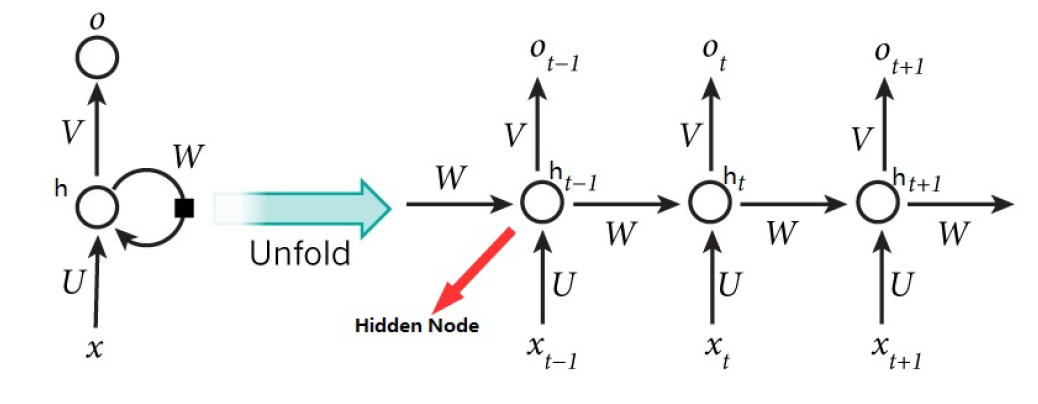
\includegraphics[width=\textwidth]{rnn}
\centering
\caption{Recurrent neural network expanding through time steps \cite{zhao}.}
\end{figure}

Recurrent neural networks (RNNs) are a type of neural network models designed for processing sequential data. The data is sequential which means it is processed in time steps by the model. This notion of time step does not have to mean literal concept of time that is used in real life. For example, it can be the position in the sequence (which is exactly the case for NLP). Since the length of a sequence can be really long, the model uses parameter sharing instead of optimizing separate parameters for each time step. This parameter sharing paradigm helps the model to generalize to different sequences by learning relationships between different time steps and different sequence lengths. Figure 2.1 shows a simple RNN and its expansion with respect to time. As it can be seen from the figure, the network produces an output in every time step.

Recurrent neural networks have numerous variants usually constructed by using different ways for connecting network layers or introducing additional computational mechanisms in order to increase generalization capability. 

\section{Long Short-Term Memory}

\begin{figure}[t]
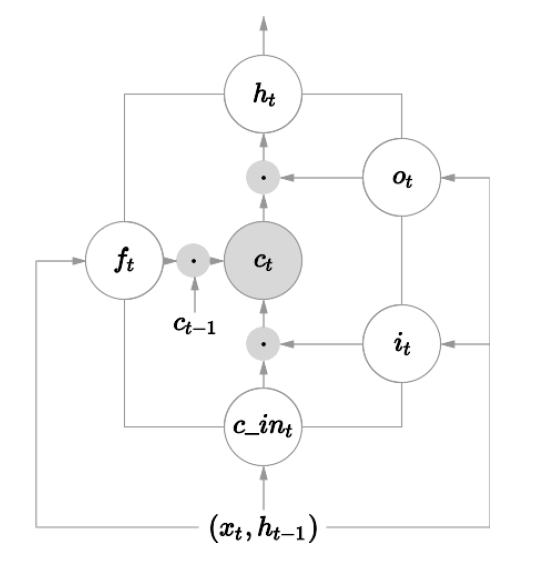
\includegraphics[scale=10]{lstm}
\centering
\caption{A typical LSTM cell \cite{paszke}.}
\end{figure}

Long Short-Term Memory (LSTM) is a variant of RNNs that adds extra computational mechanisms to the network in order to avoid the vanishing and exploding gradient problems. These computational mechanisms include a memory cell and a set of logical gates. With these modifications, the model is able to remember information for long periods of time much better than vanilla RNNs.

Especially in NLP, this is an important aspect since natural language contains context relationships between words which can be observed at different time steps. 

LSTM adds a memory cell $c_{t}$ for every time step t. At each time step t, a single unit works with the input state $x_{t}$, the hidden state $h_{t-1}$ and the memory state $c_{t-1}$ to calculate the hidden state $h_{t}$ and the memory state $c_{t}$. The memory cell has three computational mechanisms: input gate i, forget gate f, and output o. These gates are also trained meaning that their weights are updated with gradient descent with respect to time. It is known that learning these gates helps with gradient explosion.

Figure 2.2 shows a basic LSTM cell. Equations for calculating the elements of an LSTM cell are \cite{paszke}:

\begin{equation}
i_{t} = \sigma(W_{xi}xt + W_{hi}h_{t-1} + b_{i})
\end{equation}

\begin{equation}
f_{t} = \sigma(W_{xf}xt + W_{hf}h_{t-1} + b_{f})
\end{equation}

\begin{equation}
o_{t} = \sigma(W_{xo}xt + W_{ho}h_{t-1} + b_{o})
\end{equation}

\begin{equation}
c_in_{t} = \tan(W_{xi}xt + W_{hi}h_{t-1} + b_{i})
\end{equation}

\begin{equation}
c_{t} = f_{t} \odot c_{t-1} + i_{t} \odot c_in_{t}
\end{equation}

\begin{equation}
h_{t} = o_{t} \odot \tan(c_{t}) 
\end{equation}

Parameters of the above equations are:

\begin{itemize}

\item $W_{x\_}$ and $W_{h\_}$: Weights for input x and hidden state h respectively.

\item $\sigma(\_)$ and $\tan(\_)$: Element-wise sigmoid function and hyperbolic tangent function.

\item $\odot$: Element-wise multiplication.

\item b: Bias parameter.

\end{itemize}

\section{Sequence to Sequence Model Architecture}

First introduced by \cite{Vinyalsetal} neural sequence to sequence framework consists of two components, encoder and decoder. Encoder creates a low dimensional representation of the source sequence called the thought vector. It aims to capture semantical and contextual relationships of the source sequence. Then the thought vector is fed into decoder which produces a high dimensional target sequence. The process is shown in Figure 2.3. Main idea of the encoder-decoder pair is to create a mapping between words and vectors, in other words capturing the meaning as numerical vectors. By design, both encoder and decoder should be a recurrent neural network or a variant of it. In the model that is used in this work, stacked LSTM's are used for both encoder and decoder. During the decoding process, generation of new words depends on the word generated before by decoder. The decoder starts generating the target sequence when it recognizes the 'EOS' (end-of-sentence) character in the source sequence. EOS character is usually appended to the end of source sequence. The model maximizes the log probability of the target sequence given the source sequence.

\begin{figure}[t]
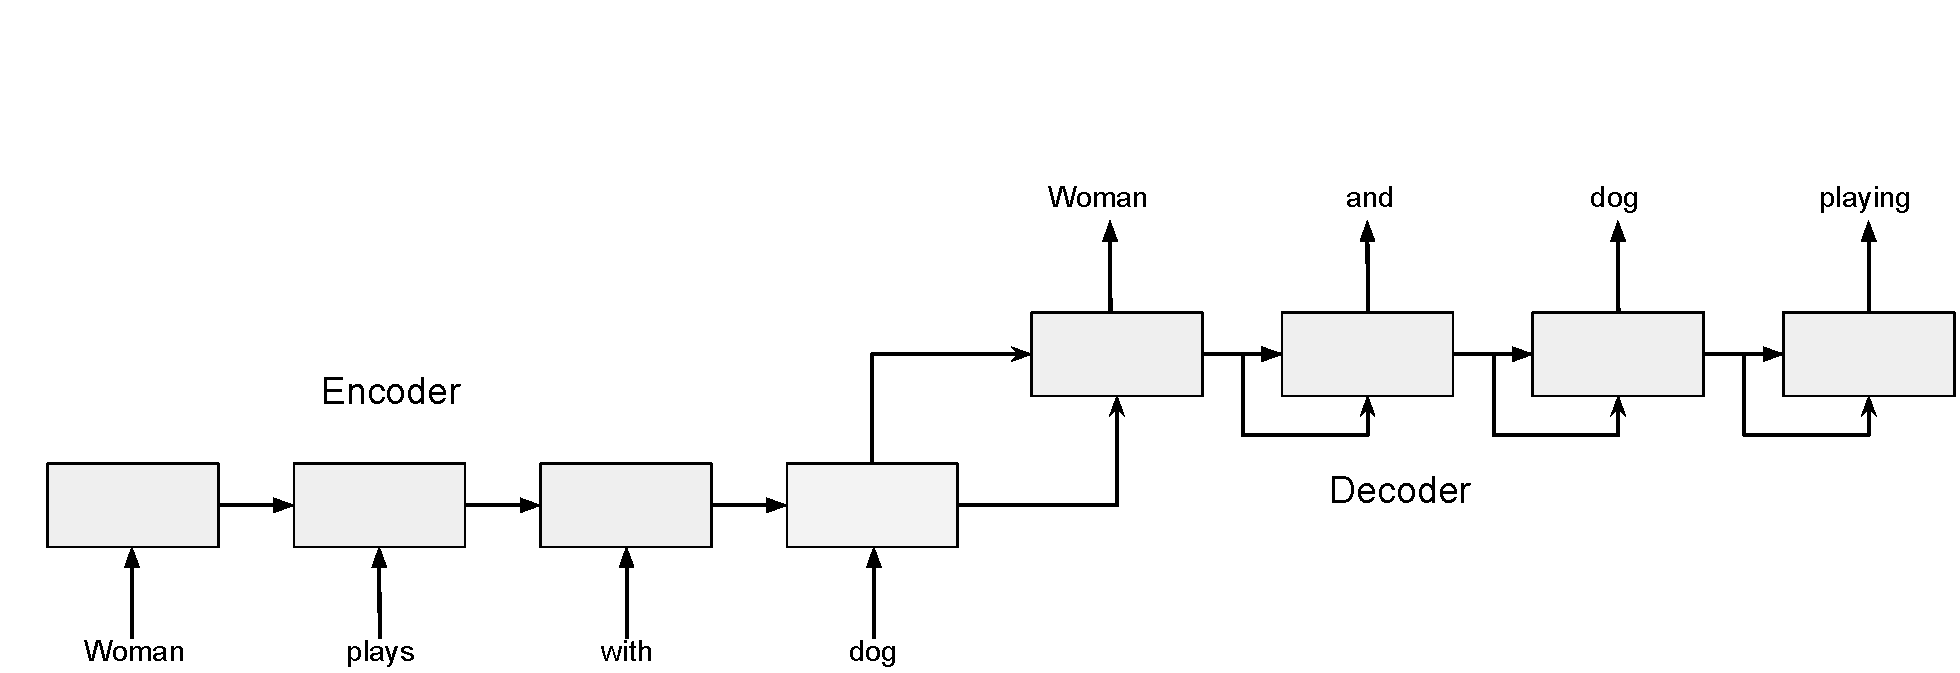
\includegraphics[scale=0.45]{seq2seq}
\centering
\caption{Sequence to sequence learning with encoder-decoder framework.}
\end{figure}

\section{Incremental Learning}

Incremental learning is a learning scheme based on training the model continuously in order to adapt to new training data without losing existing knowledge base. It is mainly used in cases where there is a data stream, constantly providing new data points. Incremental learning based models are mainly used to tackle problems like data availability and low resources. Incremental learning becomes essential in human-in-the-loop settings where the model has a feedback loop with users. Main concern of incremental learning is adaptivity since the model is especially prone to changes in the training data distribution, a situation called concept drift which is explained in previous section. 

Additionally the specification of how to adapt the model creates another problem. Depending on the task and data at hand, how the model should exactly deal with the balance between old and new information has to be decided beforehand. Many incremental learning strategies for deep neural models consists of design decisions (hyper-parameters, network topology etc.) in order to deal with this problem. For example, using a large learning rate can lead the model to quickly overwrite existing knowledge with most recent data points. In this work, some of these strategies are experimented on paraphrase generation task.

\begin{figure}[t]
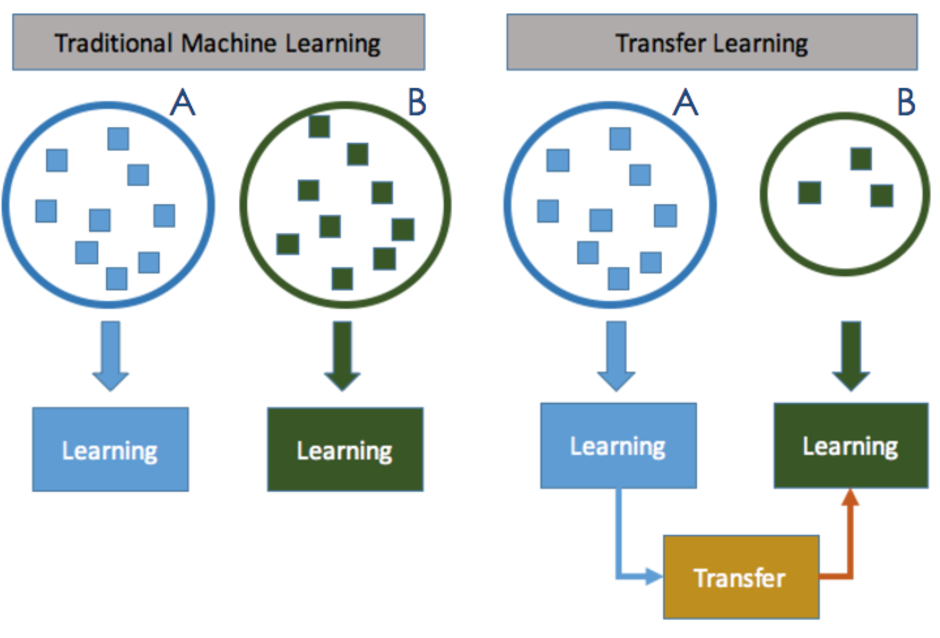
\includegraphics[width=\textwidth, height=10cm]{transfer-learning}
\centering
\caption{Idea behind transfer learning.}
\end{figure}

\section{Transfer Learning}

Transfer learning is based on the idea of using the knowledge gained from previously learned tasks and datasets. Usually it is used for decreasing the amount of training data and time of a low resource task when obtaining more training data is impractical. Moreover it is used for enhancing the generalization capabilities of an existing model, for example adding a new label for classification in image recognition task. This is a very important use case especially if the existing model is large since transferring knowledge eliminates the need of retraining the whole model. It can be also used to personalize an existing large model with a new domain specific dataset, enhancing its performance on the new domain. Figure 2.4 shows the basic workflow of transfer learning.

Deep neural models learn multiple hidden representations of the datasets, some part of which are shared between different tasks and datasets. Therefore transfer learning for deep neural models usually consists of copying layer weights across models and applying restrictions to new model in order to preserve existing knowledge. In the field of NLP, this process includes transferring learned word embeddings (numerical representations of words) and hidden layers (learned relationships of the datasets like context). Depending on the target task and dataset, the method of transfer which basically represents how the target model is trained, can significantly change. Different methods of transfer can include changing hyperparameters, freezing network layer or adding new layers.

\section{Active Learning}

Active learning is a learning scheme based on selecting training samples to be annotated by using different sampling strategies. These strategies employ certain criteria in order to create an opinion on how informative or useful a data point is and they are called sampling methods. Informativeness of a data point can depend on the dataset, task and model therefore selection of the sampling method is very crucial. The criteria considered by a certain sampling method could simply be a heuristic about the nature of dataset at hand or they can depend on the opinion of model about the data points or they can depend on feature representations of the dataset like similarity measures. Usually, sampling methods combine multiple criterions for evaluating the informativeness of a data point and some of these criteria may require complex algorithms to be obtained. 

\begin{figure}[t]
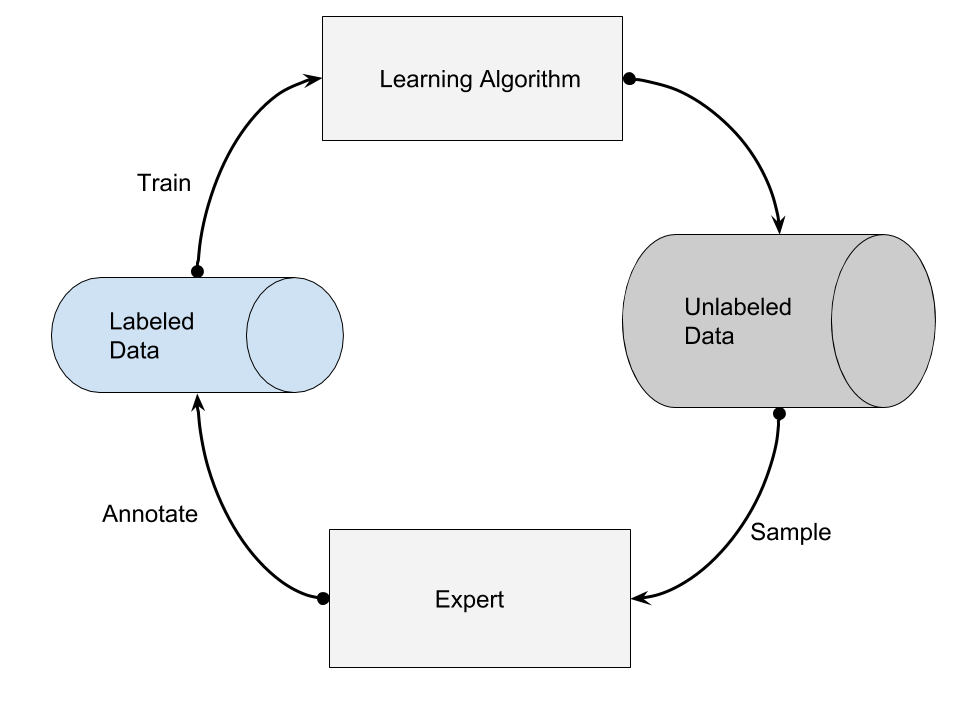
\includegraphics[width=\textwidth, height=10cm]{active-learning}
\centering
\caption{Pool based active learning scheme.}
\end{figure}

Figure 2.5 shows the basic workflow of active learning scheme. Main purpose of active learning is obtaining greater or similar performance with fewer labelled training data since collecting a large, labelled training data can be difficult, costing time and money. In our work, active learning is used as an option for enhancing human-in-the-loop data acquisition by asking the users to annotate most difficult samples. Additionally it is important to see if using adaptive learning can make the model more adaptive. It is also worth studying what constitutes an informative sample when it comes to paraphrase pairs.

\chapter{Adaptive Learning Strategies}\label{approach}

This chapter explains our approach for adaptive neural paraphrase generation. It describes the main learning strategies that are used in detail including what purpose do they serve in our human-in-the-loop setting. First, details of the model which are used in the experiments are explained. Then descriptions of the datasets and the evaluation metric are presented. For last, the learning strategies and the experimental setups are discussed.

\section{Model Details}

In this work, a lightweight variant of the model proposed in  \cite{Prakashetal} with bahdanau attention \cite{bahdanau} is used. The reason the exact same model from the paper is not used is to fully explore all learning strategies since even with a lightweight version of the model, training takes a long time. The model keeps the same stacked LSTM based multi-layer architecture with residual connections but using 3 layers instead of 4. Figure 3 shows the basic unit in the model.

\begin{figure}[t]
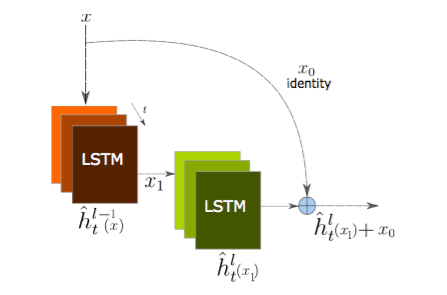
\includegraphics[width=\textwidth]{residualLSTM}
\centering
\caption{Stacked LSTM based model \cite{Prakashetal}.}
\end{figure}

During experiments, the model has 512 units in each LSTM layer with dropout probability of 0.3 after each layer. The model trains its own word embeddings with the embedding size of 512. For all experiments learning rate is started with 0.001 and decayed exponentially, with the square root function.

In the cases when it improves the performance, a beam search with beam size of 5 is used.

\section{Datasets and Evaluation Metric}

Four different datasets are used in the experiments varying in context and complexity. 

The Microsoft Research Paraphrase Corpuus (MSR) \cite{msrp} is a small but very challenging dataset which contains 5800 pairs of paraphrases extracted from news sources. Since the paraphrase pairs are extracted from different news sources the dataset contains a lot of lexical and contextual variety. It also contains a lot of special words and concepts. Because of these reasons MSR corpus is a very hard dataset to create paraphrases from even by the state-of-the-art model with high computational resources. The dataset is separated into subsets of 2753, 997 and 150 for training, test and validation respectively.

The Quora Question Pairs (QUORA) is a dataset consisting of question pairs which are labeled as paraphrases. It is originally a dataset for paraphrase recognition not paraphrase generation. The positive class of dataset is filtered and 155,000 paraphrase pairs are collected. There are one to many relationships in the dataset which means it contains multiple paraphrases for same source text. This property makes the dataset an ideal candidate for paraphrase generation. The dataset is separated into subsets of 119445, 22861 and 2000 for training, test and validation respectively.

The Microsoft Common Objects in Context (MSCOCO) \cite{mscoco} is a large dataset consisting of human generated image captions with 351,163 pairs. It also has one to many relationships. MSCOCO is one of the most popular datasets used in paraphrase generation literature. All of the dataset is used for training.

The PPDB Lexical (PPDB) \cite{ppdb} is a large dataset which contains 500,000 pairs of short paraphrases and it is also very popular in paraphrasing research. The paraphrases in this dataset are short that lack context information. All of the dataset is used for training.

\begin{table}
\small
 \begin{tabular}{||c c c c||} 
 \hline
 Label & Sentence & Dataset & \\ [0.5ex] 
 \hline
 source & the dvdcca then appealed to the state supreme court & MSR & \\
 \hline
 target & the dvd cca appealed that decision to the us supreme court & MSR & \\
  \hline
 source & why do rockets look white & QUORA & \\
 \hline
 target & why are rockets and boosters painted white & QUORA & \\
 \hline
 source & a blue and white bathroom with butterfly themed wall tiles & MSCOCO & \\
 \hline
 target & an angled view of a beautifully decorated bathroom & MSCOCO & \\
 \hline
 source & despicable & PPDB & \\
 \hline
 target & contemptible & PPDB & \\
 \hline
\end{tabular}
\caption{Example paraphrase pairs from the datasets.}
\end{table}


Table 3.1 shows example paraphrases from all the datasets used in the experiments. As it can be seen from the table, the datasets are varying in paraphrase complexity therefore it is easy to see why MSR dataset is harder to paraphrase than the others. MSR and QUORA datasets are used as target datasets on which the model is built and evaluated whereas MSCOCO and PPDB are used as source datasets for transfer learning.

There are no evaluation metrics especially designed for paraphrase generation. Therefore for evaluation the metric BLEU \cite{Papinenietal}  is used. BLEU is a widely used metric for paraphrase generation even though it is designed for machine translation. It is seen as a suitable option for paraphrase generation since it is shown that the score correlates well with human evaluation.

\section{Experimental Setups}

The human-in-the-loop data acquisition process is simulated by randomly dividing a dataset into train, test and validation, taking training set's subsets and feeding it to the model in each iteration. After each iteration the model is trained with the data available according to learning strategy which is experimented on and evaluate its performance iteratively with the test set. The test set is preferred to be relatively large in order to test how well the model generalize after each iteration. The model is trained with same amount of epochs and start the training with same hyperparameter configurations through the iterations in order to compare the performance without bias. If it is necessary, parameter tuning is done on validation set beforehand and the best model is taken for the experiments with learning strategies. Every learning strategy is experimented with the same model (same architecture, same hyperparameters etc.).

\section{Incremental Learning Strategies}

In the continuous setting this thesis studies, the training data is limited at the beginning. After a certain amount of time, the system is able to collect enough data to build a stable model with supervised learning. This model then, can be used for application purposes as long as it performs at an acceptable level. There are two major drawbacks in this solution. Firstly, the model is not able to use the training data which is collected after its creation. This is clearly a waste of resources since the training data comes from a continuous stream. Secondly and most importantly, the model would have to be trained on a regular basis just to keep up with the new training data. This is not desirable and not practical even impossible depending on the circumstances. Therefore, incremental learning is a natural option in this case.

The main concern in human-in-the-loop setting is to make continual, data-driven learning possible since traditional supervised learning is not practical. The model should keep learning with incoming training data which is provided by the data stream, adapt itself to the changes in dataset without forgetting the knowledge it learned before. Since the model is getting training data in small chunks, one of the most important design decisions which has to made is how to process available training data through time. In case of neural models learning basically means to update model's weights by iterations according to the training data. Because of the very nature of gradient descent based learning the more certain data points are used in training the more the model is going to adjust itself towards to those data points. This could lead to a bias towards the training data which is gathered at past, severely hurting the model's learning capability. It is important to notice that this can also happen within the same dataset if the dataset has high variance. This problem would not occur if the model is trained with supervised learning since the whole dataset would be available for training.

As explained in previous sections, concept drift is the other big challenge that has to be considered when learning in continuous data streams. Optimally model should be able to pick up the statistical and conceptual changes in the incoming training data and update its weights accordingly. The model should be able to do this without forgetting previously learned knowledge so that it can preserve its original functionality. After adapting to the new training data, it should still be able to perform reasonably well when it encounters test data from the original dataset. 

It is reasonable to say that when the two problems described above are considered, adaptivity of a model is basically a tradeoff between how fast it learns the new knowledge and how fast it forgets the old one. Any learning strategy that is to be used in adaptive learning, should employ some measures in order to preserve the balance between learning and forgetting. As it is said before because of the very nature of how deep neural models learn, it is impossible to avoid either one of them but it is possible control the rate of how fast the model learns and forgets.

Two different incremental learning strategies which differ in how they process the incoming training data, are proposed and experimented with. The model is regulated with different methods available in traditional supervised learning. The behaviour of these two incremental learning approaches are studied and some insights on adaptive paraphrase generation, are provided. The training and regularization methods that are used, are fairly simple but they haven't been studied before so the finding of this thesis is thought as a foundation for more complex approaches for adaptive learning in NLP.

\subsection{Incremental Learning with Data Pooling (IL1)}

The first learning strategy trains continuously (weights are not re-initialized between iterations, model uses and updates the same weights) from a data pool which contains all the data collected in previous iterations. The model uses all the data available to it regardless how old or new the data is. Figure 3.2 shows the basic work flow of the learning strategy. As it can be seen from the figure at the end of each iteration, the collected data is placed in a data pool and the model trains itself using the updated data pool. After the training process next iteration starts and cycle continues. The purpose of this learning strategy is mainly show that if the neural model can constantly improve itself through time to the incoming data. Main focus is not to forget previously attained knowledge while learning new training data reasonably well and make model to use all the resources available. The advantages of this learning strategy can be listed as:

\begin{figure}[t]
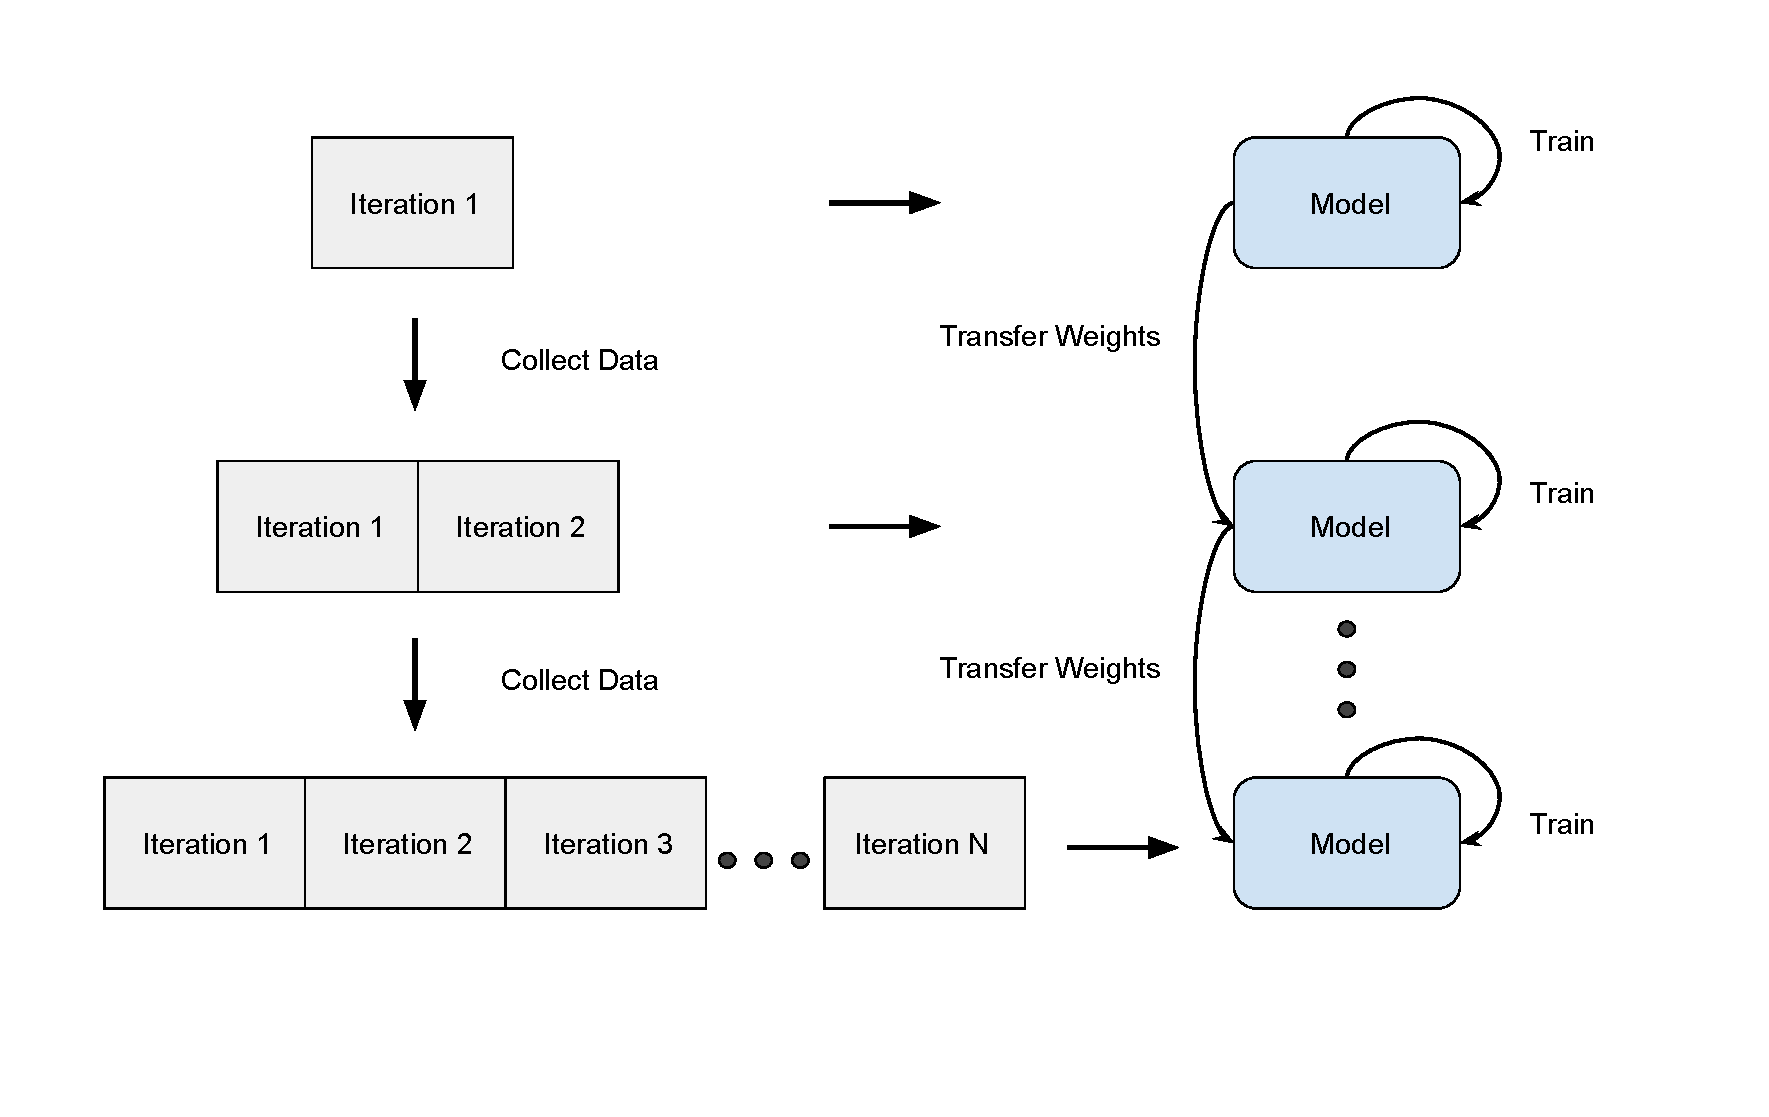
\includegraphics[width=\textwidth]{IL1}
\centering
\caption{Incremental learning with data pooling (IL1). The model uses data from all prevous iterations, hyperparameters re-initialized and weights are transferred through iterations.}
\end{figure}

\begin{itemize}

  \item Since the model trains on all data available at the end of each iteration, it is unlikely to forget learned knowledge from previous iterations.
  \item The model has the chance to learn more difficult data points better especially if they are encountered in early iterations. Basically instead of waiting to get enough data to learn with supervised learning, that time can be used to work on challenging data points seen by the model.

\end{itemize}

The disadvantages of this learning strategy are:

\begin{itemize}

  \item Since the size of data pool is increasing linearly, the time model takes to the end of each iteration and the required memory for data pool, increases as well. This increase can be linear or exponential depending on the model.
  \item The model sees data points from earlier iterations way more often which means it updates its weights according to those data points more often. This can cause overfitting to those particular data points which can diminish the performance of the model.

\end{itemize}

\subsection{Incremental Learning without Data Pooling (IL2)}

The second learning strategy trains continuously (weights are not re-initialized between iterations, model uses and updates the same weights) only from the data of last iteration. There is no data pool that aggregates collected training data. Figure 3.3 shows the basic work flow of the learning strategy. As it can be seen from the figure, the model only updates itself with the most recent iteration. After the training process next iteration starts and cycle continues. Purpose of this learning strategy is to create an efficient model in terms of the training time and memory. The main focus is the adaptivity of model to new data. The advantages of this learning strategy can be listed as:

\begin{figure}[t]
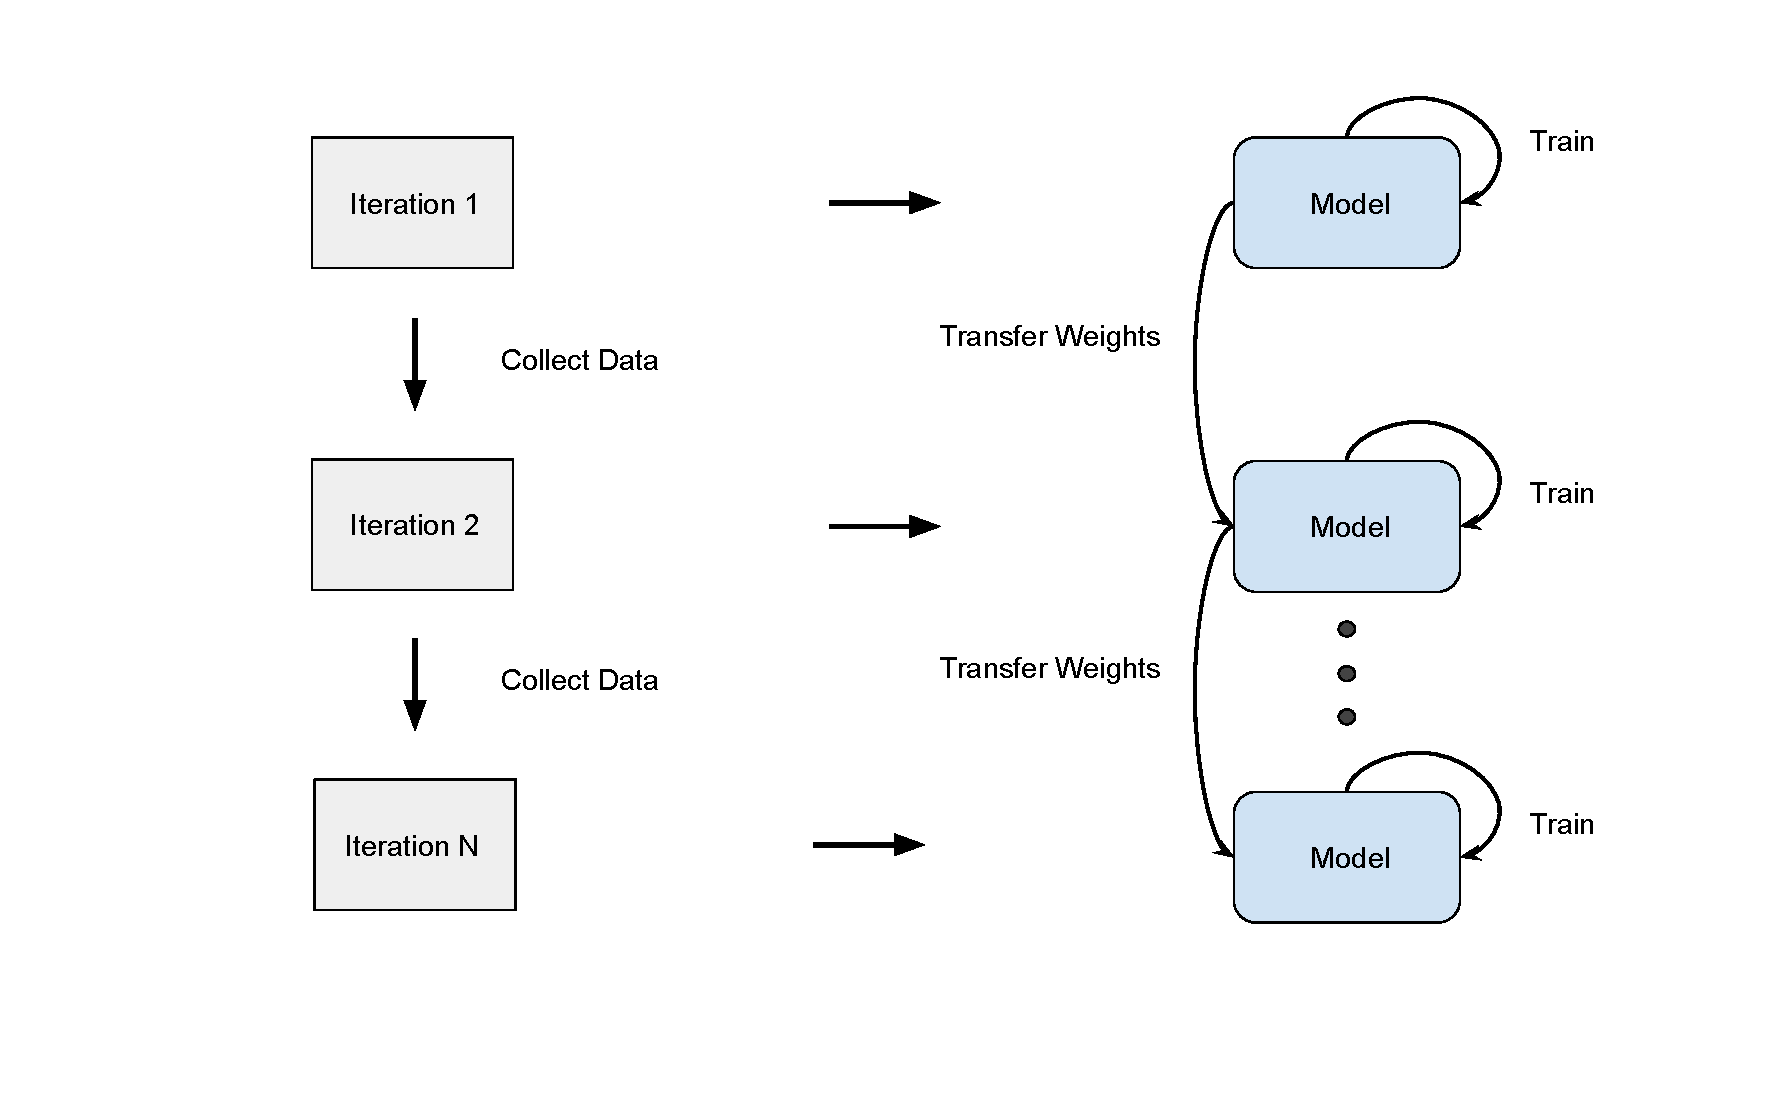
\includegraphics[width=\textwidth]{IL2}
\centering
\caption{Incremental learning without data pooling (IL2). The model only uses data from latest iteration, hyperparameters re-initialized and weights are transferred through iterations.}
\end{figure}


\begin{itemize}

\item Since the size of data pool is constant, it is efficient in terms of time and memory.
\item The model sees all data points for equal amount of times therefore it does not have the problem of overfitting as incremental learning with data pooling.

\end{itemize}


The disadvantages of this learning strategy are:

\begin{itemize}

\item Since the model trains on iterations separately it is prone to overwrite and forget old knowledge from previous iterations.
\item All training points are updated for same amount of iterations. If the number of epochs are not large enough the model can underfit and fail to generalize.

\end{itemize}

\subsection{Incremental Learning with Network Expansion (IL-NE)}

The last learning strategy trains continuously (weights are not re-initialized between iterations, model uses and updates the same weights) and expands the neural network after certain number of iterations. In this context network expansion means adding another LSTM layer to the network. Purpose of this learning strategy is to increase adaptive capabilities of the model. Main focus is to deal with possible concept drift which can occur during data acquisition. By adding randomly initialized new layers when more than a certain amount of data is introduced to the model, specialized layers focusing on old and new information are aimed to be created. Experiments are conducted with expansion in every third iteration and expansion only in the fifth iteration. Additionally, an experiment is done with freezing first active layer in every expansion step, studying if restricting the model through time helps with adaptivity.   

\subsection{Incremental Learning Baseline (IL3)}

The model is also trained from ground zero (with the weights re-initialized) from data pool at the end of every iteration in order to create a comparable baseline. The baseline model which is trained after the last iteration is basically the model trained with supervised learning since it uses the whole training data available. The basic idea is to check if the incremental learning strategies achieve better or comparable performances than last baseline model. Figure 3.4 shows how the baseline is created.

\begin{figure}[t]
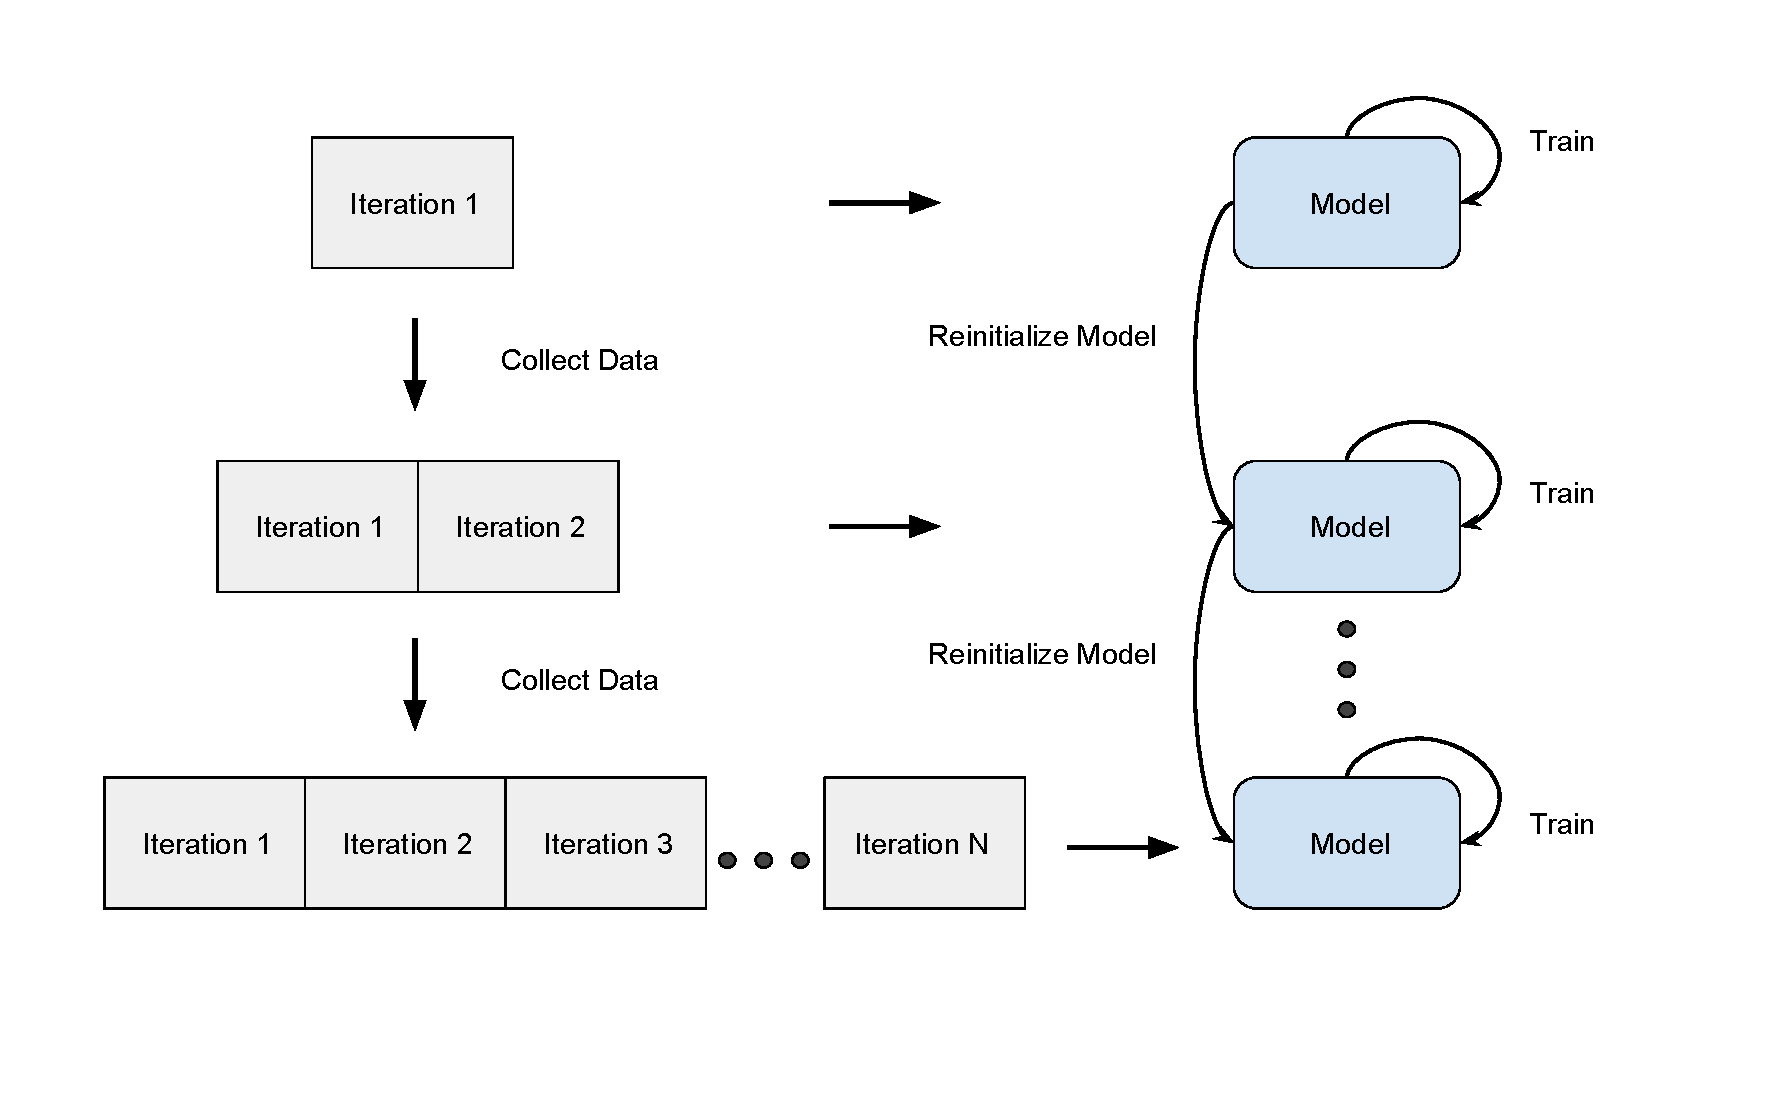
\includegraphics[width=\textwidth]{IL3}
\centering
\caption{Incremental learning baseline (IL3). The model is trained from scratch for each iteration, no knowledge transfer involved.}
\end{figure}

\subsection{Model Regularization in Incremental Learning}

Simple and well known regularization techniques are used with incremental learning strategies in order to control the tradeoff between old and new information. The regularization techniques that are used in the models are dropout, learning rate decay and layer freezing. Learning rate and its decay is used to control how large the weight updates are during the learning. A non-shared regularization mechanism is employed where every iteration has its hyperparameters re-initialized in order to make the model adaptive to most recent data. In other words while the weights of the network is transferred through iterations, the decayed learning rates are not.

In this case the assumption is a very small learning rate with high decay rate will make the model unresponsive to the latest iterations. Exponential learning rate decay (square root decay) is used in our experiments which means the learning rate will decrease through iterations. Dropout is used to prevent overfitting especially in incremental learning with data pooling where the model is updated for certain data points way more than the rest of dataset. Also a certain number of the layers are freezed so that corresponding layers' weights are not updated during training. The idea is to make sure that some of the previously learned knowledge is not overwritten by the incoming dataset. 

\section{Transfer Learning Strategies}

During incremental learning, the model is trained at the end of each iteration with training data specified by the chosen incremental learning strategy. Since the model is trained continuously without reinitializing the weights in each iteration, this is equivalent to transfer learning between iterations. In the initial experimental setups, the training data comes from the same dataset divided into subsets provided as iterations. This experiment setup is expanded by transferring knowledge from a different paraphrasing dataset and start the incremental learning process with a pre-trained model or in other words with a knowledge base. 

Transfer learning from other sources are extremely relevant to the continuous human-in-the-loop setting especially in the cases where there are no resources to collect a large dataset. Since the training data is collected iteratively the model would have to work with even smaller dataset at the beginning. Transfer learning can help the model to learn better, providing a better initialization in the worst case scenario and increase the performance in this case. 

More importantly by training a model in a different dataset and using the pre-trained model to learn a new dataset, an artificial equivalent of concept drift is simulated no matter what transfer strategy is used. Basically in this case, there is a model which is used for a different dataset (different statistics, distribution, context etc.) than the one it is trained with. Only difference between this scenario and the concept drift scenario that exists in incremental learning is, in this case the model has access to all of the new dataset, instead of small chunks. Therefore finding good strategies for transfer learning can help with the concept drift problem if the transfer strategies is combined with incremental learning. 

Before starting with the transfer learning from other paraphrase datasets, experiments are conducted for answering these questions:

\begin{itemize}

\item Is knowledge transfer possible for neural paraphrase generation?

In order to answer this question, a model is trained with a large paraphrasing dataset as a source model. Then the transfer is done from this source model to target model with simplest way possible which is copying the weights of every component of source model and train the target model in a supervised manner. The performance is compared with traditional supervised learning without transfer to see if there is any improvement.

\item If answer to the first question is yes, what components of the model are being transferred?

To see what aspects of the source model is transferred, the experiments are run with three different settings; transfer embedding layer only, transfer embedding and hidden layers, transfer all layers including output layers. The performances are compared to see what components lead to improvement. 

\item Does transfer success depend on the characteristics of the participant datasets?

In order to speculate about what properties of the datasets relevant to knowledge transfer, experiments with three different source datasets and two target datasets, are run. The transfer performances are studied to establish some correlations between performance and properties like context, content, size of the datasets.

\end{itemize}

After establishing knowledge transfer is indeed possible, three different transfer strategies are proposed:

\begin{itemize}

\item INIT: Knowledge transfer is done by copying every component of source model to target model.  

\item Freeze n-layers: Same as INIT but first n layers of the model are freezed.

\item Surplus layer:  Same as INIT but a surplus layer is added before output layer and all the other layers are freezed.

\end{itemize}

Basically, proposed transfer strategies are designed for putting restrictions on the target model, directly effecting how much the model learns from training data. Whereas INIT puts no restrictions on the target model, surplus layer conservatively keeps the knowledge from source model and freeze n-layers approach is thought as a middle ground between them, making adjustments between knowledge learned from source dataset and target dataset . With transfer learning the model deals with a similar old vs. new knowledge tradeoff as incremental learning but with a different scale. In this case old knowledge part of the tradeoff is much larger and can have significant effects on the models performance. Moreover all of the transfer strategies proposed in this chapter are designed while specific use cases are considered. It is hypothesized that INIT is more suitable when the dataset for target model is large and the model has to be complex whereas surplus layer is more suitable when the dataset for target model is small and the model has to specialize (general to specific for the same domain). 

The same regularization techniques used for incremental learning strategies are used for transfer learning strategies as well, even though their effect on the performance can be not the same. Since it is essential to efficiently use the knowledge learned from the source dataset in the target dataset, learning rate for the target model becomes very important. A large learning rate might overwrite the existing weights very quickly which means losing the information gained before. Therefore in the experiments, a larger learning rate is used for source dataset and smaller learning rate is used for target dataset. The same exponential learning decay that is used in incremental learning, is kept.

\section{Active Learning Strategies}

Active learning is perfectly suitable for human-in-the-loop setting since it aims to enable learning with less amount of data. Not only it can reduce the cost of data acquisition, it can also enhance the overall process since it enables the model to learn faster which would mean earlier and more meaningful involvement with the users. As it is explained before the core idea behind active learning is determining the most difficult data points to paraphrase and make the users annotate those data points. The aim is to integrate active learning into the incremental learning with data pooling strategy and study its effects on the model's performance. It is hypothesized that since incremental learning with data pooling updates its weights towards to some data points in the dataset more than others, if those points are made sure to be most difficult data points to paraphrase, this can help the model to train better and faster.

It is hard to define a difficult or informative data point in case of paraphrase generation just because of the fact that it is a generation task not classification or regression. Contrary to other NLP tasks like paraphrase recognition or named entity recognition, in paraphrase generation the model only has the source texts to work with which limits the information it has on the dataset. For example in the case of paraphrase recognition, the dataset contains both of the paraphrase pairs and the annotator is only have to decide if they have the same meaning or not but nevertheless information from both of the sentences can be used for sampling. In this case, the sampling strategies which consist of heuristics regarding the training data, are based on only the source texts. Three different sampling strategies are combined with incremental learning with data pooling. Sampling techniques that are used for the experiments are:

\begin{itemize}

\item Random Sampling (RS): Sentences which are going to be paraphrased by the user are selected randomly. This is the default method for all of the other experiments in this thesis and used as a baseline.

\item N-gram Coverage (NC): Proposed in \cite{rubio} for interactive machine translation, this sampling technique focuses on selecting the rarest data points in terms of their n-grams. In other words, this technique aims to calculate how much new information a data point can provide. The hypothesis is rarest sentences have to be seen more for model to learn an accurate probability estimation. 

Before the training, number of each n-gram present in the training data is calculated and stored. Since human-in-the-loop approach is simulated, n-gram counts of the whole dataset can be calculated beforehand but in a real world application where new training data is constantly streamed, they should be updated after each iteration. An n-gram is labelled as rare when it appears less than A times in training data. Using this label, the score for a given source sentence f, is computed as:

\begin{equation}
C(f) = \frac{\sum_{n=1}^N \lvert{\nu^{<A}_{n}(f)} \lvert} {\sum_{n=1}^N \lvert{\nu_{n}(f)} \lvert} 
\end{equation}


where ${\nu_{n}(f)}$ is the set of n-grams with size n in f, ${\nu^{<A}_{n}}$ is the set of n-grams of size n in f that are rare and N is the maximum n-gram order. In experiments with incremental learning with data pooling, N = 4 is chosen as the maximum n-gram order and a value of 10 is chosen for the threshold A. In order to asses how well n-gram coverage represents the informativeness of data, an experiment is conducted with reverse n-gram sampling where the data points are chosen based on how frequent they are in the dataset in terms of n-grams. The score for reverse n-gram sampling is calculated as:

\begin{equation}
C(f) = \frac{\sum_{n=1}^N \lvert{\nu^{>=A}_{n}(f)} \lvert} {\sum_{n=1}^N \lvert{\nu_{n}(f)} \lvert} 
\end{equation}

where the terms are the same as n-gram sampling equation.

%\item Least Confidence (LC): A very intuitive sampling technique, it chooses data points in which the model has least confidence in. In the context of deep neural models this means to select the data points that are assigned with lowest probability according to the equation \cite{shen}:
%
%\begin{equation}
%1 - \max_{y_{1}.....y_{n}}  \mathbb{P}  \left[ {y_{1}.....y_{n}}  | \{ x_{ij} \}  \right]   
%\end{equation}
%
%For LSTM based sequence-to-sequence model used in this work, the score for a data point is calculated by using the probability of greedily decoded sequence.

\end{itemize}

Since MSR dataset contains a very small number of paraphrases, active learning strategies are only tried on QUORA dataset.




\chapter{Results}\label{results}

This chapter reports the results of experiments done with the proposed learning strategies and discusses the findings. First, evaluations of each strategy are given separately followed by the experiments which evaluates the combinations of different strategies. At the end, an overall discussion of the results is given.

\begin{table}[t]
\centering
\small
 \begin{tabular}{|c | c | c | c | c | c | c | c | c | c |} 
 \hline
 \% & 20 & 30 & 40 & 50 & 60 & 70 & 80 & 90 & 100 \\ [0.5ex] 
 \hline
  IL1 & 0.1 &  \textbf{0.92} &  \textbf{0.94} &  \textbf{1.56} &  \textbf{1.13} &  \textbf{1.11} &  \textbf{1.26} &  \textbf{1.37} &  \textbf{1.41}  \\ 
 \hline
  IL2 & 0.07 & 0.15 & 0.21 & 0.47 & 0.77 & 0.99 & 1.04 & 1.19 & 1.16 \\ 
 \hline
 Baseline & \textbf{0.12} & 0.27 & 0.6 & 1.32 & 0.96 & 1.08 & 1.24 & 1.26 & 1.34 \\ 
 \hline
 SL & - & - & - & - & - & - & - & - & 0.09  \\ 
 \hline
\end{tabular}
\caption{BLEU scores of incremental learning on the MSR dataset. Each column represents an iteration, first row shows what percent of the dataset is used in that iteration. Each row except the last represents the performance of a particular learning strategy which is described in Chapter 3. The last row represents the results from \cite{brad}.}
\label{table:4.1}
\end{table}

\section{Neural Paraphrase Generation with Incremental Learning}

Table 4.1 presents the results of incremental learning strategies on the MSR dataset. The model is highly sensitive to parameter tuning, failing to converge with high learning rates. The model is trained on a validation set with different hyperparameter configurations, mainly with different dropout probabilities and learning rates, and the configuration with the best performance is used in the experiments. As it can be seen from the table, the model performs very poorly, achieving a BLEU score of 1.34 with traditional supervised learning. This poor performance might be related to the dataset's small size and high complexity. Moreover a result from \cite{brad} is also reported in order to reinforce the difficulty of MSR dataset. Their model achieved a BLEU score of 0.09 on the MSR dataset with supervised learning. 

Incremental learning with and without data pooling achieve BLEU scores of 1.41 and 1.16 respectively. It can be seen that all of the learning strategies including the baseline, seem to improve over time increasing their performance in a steady fashion at every iteration even though there are anomalies in baseline and incremental learning with data pooling, at the 4th iteration with 50 percent of the data. It is also observed that when trained with data pooling in an incremental manner, the model performs slightly better than supervised learning. Nevertheless the model fails to generate meaningful and grammatically correct paraphrases in every case.

Even though a clear pattern through iterations can be seen, the results of this experiment is not conclusive due to model's very poor performance. Moreover the high variance between different runs highly suggest that the results are not meaningful and the neural network is basically modelling noise. Each learning strategy has been run 3 times and the variance of the best performing learning strategy which is the incremental learning with data pooling, is 0.617. This a very high number compared to actual BLEU scores achieved by the model. 

At the end it is clear that generating coherent paraphrases for MSR dataset is impractical if it is not impossible for our model. Moreover it is not applicable to human-in-the-loop setting since it basically produces noise in early iterations. This severely undermines the involvement of model with the data acquisition process, in other words the model is unable to make meaningful suggestions to the user.

\begin{table}[b]
\centering
\small
 \begin{tabular}{|c | c | c | c | c | c | c | c | c | c |} 
 \hline
 \% & 20 & 30 & 40 & 50 & 60 & 70 & 80 & 90 & 100 \\ [0.5ex] 
 \hline
  IL1 & 10.49 &  \textbf{19.43} & \textbf{21.91} &  \textbf{23.30} &  \textbf{24.30} &  \textbf{24.50} &  \textbf{25.15} &  \textbf{25.45} &  \textbf{26.19}  \\ 
 \hline
  IL2 &  \textbf{10.68} & 17.58 & 18.79 & 19.06 & 19.50 & 19.46 & 19.35 & 19.54 & 19.70 \\ 
 \hline
 Baseline & 7.93 & 15.37 & 17.58 & 19.73 & 21.20 & 21.63 & 22.49 & 23.12 & 23.43 \\ 
 \hline
 SL & - & - & - & - & - & - & - & - & 22.90  \\ 
 \hline
\end{tabular}
\caption{BLEU scores of incremental learning on the QUORA dataset. Each column represents an iteration, first row shows what percent of the dataset is used in that iteration. Each row except the last represents the performance of a particular learning strategy which is described in Chapter 3. The last row represents the results from \cite{Guptaetal}.}
\label{table:4.2}
\end{table}

Table 4.2 presents the results of incremental learning strategies on the QUORA dataset. Other than a small grid search on the validation dataset with supervised learning, no hyperparameter tuning is done on the model during this experiment. As it can be seen from the table, in every case the model performs reasonably well at the end of last iteration. The baseline model with traditional supervised learning achieves a BLEU score of 23.43 and it is able to generate meaningful, grammatically correct paraphrases. The result from \cite{Guptaetal} is also reported. Their model achieved a BLEU score of 22.9 on the QUORA dataset with supervised learning. It is important to state that the training set used in this experiment is slightly larger than the reference work. Additionally a much larger test set is used in this work. Therefore it is not possible to make conclusive statements regarding the comparison of two models. Nevertheless the comparison at least shows that our model performs comparably to the other state-of-the-art approaches.

\begin{table}[t]
\centering
\small
 \begin{tabular}{|c | c | c | c | c | c | c | c | c | c |} 
 \hline
 \% & 20 & 30 & 40 & 50 & 60 & 70 & 80 & 90 & 100 \\ [0.5ex] 
 \hline
  0 & \textbf{10.68} & 19.13 & 20.45 & 20.83 & 20.44 & 20.47 & 20.78 & 20.31 & 21.11  \\ 
 \hline
  0.3 & 10.49 & \textbf{19.43} & \textbf{21.91} & \textbf{23.30} & \textbf{24.30} & \textbf{24.50} & \textbf{25.15} & \textbf{25.45} & \textbf{26.19} \\ 
 \hline
  0.5 & 8.48 & 17.05 & 19.62 & 21.58 & 22.93 & 23.26 & 23.92 & 24.58 & 25.09 \\ 
 \hline
\end{tabular}
\caption{BLEU scores of incremental learning with data pooling on the QUORA dataset with different dropout probabilities. Each column except the first represents an iteration, first row shows what percent of the dataset is used in that iteration. First column represents the dropout probabilities.}
\end{table}

Incremental learning with data pooling achieves a BLEU score of 26.19 at the last iteration, outperforming other strategies including supervised learning. Moreover it starts outperforming traditional supervised learning which uses all of the dataset, only with 60 percent of the dataset. The model starts adapting and improves its performance constantly through iterations. Even with using only half of the dataset, the model can provide reasonable paraphrases. 

The comparison between baseline incremental learning and incremental learning with data pooling indicates the reasons why data pooling performs better. From the perspective of individual iterations with both learning strategies, the model trains with the same number of epochs and same amount of data. Only difference between two learning strategies is, in incremental learning with data pooling the model employs transfer learning inside the same dataset by not reinitializing its weights in every iteration contrary to baseline incremental learning. In other words the model that is trained in a particular iteration, is already fine tuned with respect to a specific portion of the dataset. The results show that the model is able to utilize the information gained in the previous iterations.

As stated in Chapter 3, the main concern about the incremental learning with data pooling strategy is overfitting to data points which are collected in earlier iterations. Considering how prone the neural models are for overfitting, this would be an expected situation but the results show that the model does not overfit when it is trained incrementally with data pooling. Training error of the model decreases and stabilizes through epochs. It can be hypothesized that the regularization methods that are employed, are preventing the model to overfit and making the learning process stable. In order to confirm this an experiment with different dropout probabilities is done and the model's behaviour in the incremental learning setting is reported. Table 4.3 shows the effect of different dropout probabilities on the incremental learning with data pooling.

As it can be seen from the table, the model is able to learn with the dropout probabilities of 0.3 and 0.5 while it fails to adapt when there is no dropout. Even though training error decreases steadily in every iteration, the model can not improve on the test set, overfitting over time which is the expected behaviour. The incremental learning baseline is also trained with different dropout probabilities. The results are shown in Table 4.4. As it can be seen from the table, the model does not overfit even though no dropout is used.

\begin{table}[t]
\centering
\small
 \begin{tabular}{|c | c | c | c | c | c | c | c | c | c |} 
 \hline
 \% & 20 & 30 & 40 & 50 & 60 & 70 & 80 & 90 & 100 \\ [0.5ex] 
 \hline
  0 & \textbf{10.59} & 15.27 & 19.20 & 19.69 & 21.60 & 18.69 & 22.37 & 22.86 & 23.09  \\ 
 \hline
  0.3 & 7.93 & \textbf{15.37} & \textbf{17.58} & \textbf{19.73} & \textbf{21.20} & \textbf{21.63} & \textbf{22.49} & \textbf{23.12} & \textbf{23.43} \\ 
 \hline
  0.5 & 8.19 & 13.34 & 15.33 & 17.09 & 18.36 & 19.05 & 20.09 & 20.94 & 21.54 \\ 
 \hline
\end{tabular}
\caption{BLEU scores of incremental learning baseline on the QUORA dataset with different dropout probabilities. Each column except the first represents an iteration, first row shows what percent of the dataset is used in that iteration. First column represents the dropout probabilities.}
\end{table}

Incremental learning without data pooling achieves a BLEU score of 19.70 at the last iteration. The results show that even though the model improves its BLEU score in first 4 iterations it fails to adapt afterwards achieving similar BLEU scores for last 5 iterations. The model has the highest score in last iteration like the other learning strategies but increase in performance is not notable. Moreover at the last iteration, incremental learning without data pooling performs worse than both incremental learning baseline and incremental learning with data pooling.

\begin{table}[b]
\centering
\small
 \begin{tabular}{|c | c | c | c | c | c | c | c | c | c |} 
 \hline
 \% & 20 & 30 & 40 & 50 & 60 & 70 & 80 & 90 & 100 \\ [0.5ex] 
 \hline
  5 & 10.68 & 17.58 & 18.79 & \textbf{19.06} & \textbf{19.50} & \textbf{19.46} & \textbf{19.35} & \textbf{19.54} & \textbf{19.70}  \\ 
 \hline
  10 & 17.07 & \textbf{18.62} & \textbf{18.83} & 18.54 & 18.76 & 19.12 & 19.15 & 19.45 & 19.69 \\ 
 \hline
 15 & \textbf{18.96} & 18.07 & 18.47 & 18.46 & 18.87 & 19.05 & 19.11 & 19.15 & 19.19 \\ 
 \hline
\end{tabular}
\caption{BLEU scores of incremental learning without data pooling on the QUORA dataset with different number of epochs. Each column except the first represents an iteration, first row shows what percent of the dataset is used in that iteration. First column represents the number of epochs.}
\end{table}

When compared to baseline incremental learning, it is easy to see that at the last iteration both models are trained the same number of epochs. The baseline model is outperformed by the model trained with incremental learning without data pooling in the first 3 iterations but starting with the 4th iteration, it begins to outperform the other. This is an expected result because the continuous model has better weight initialization when there is not enough training data for the model to learn properly.

Both of the incremental learning strategies that are proposed, use transfer learning in the same dataset only difference being the resources they transfer from. Incremental learning with data pooling not only uses more training data to transfer between iterations, it also updates certain parts of the datasets more. It can be argued that the reason behind the low performance of incremental learning without data pooling is the fact that it is not updating the models' weights enough, hence underfitting to the whole dataset. An experiment with different number of epochs per iteration is done in order to test this theory. The results are shown in Table 4.5.

As it can be seen from the table, the number of epochs used in training does not effect the performance significantly. The model trained with number of epochs of 5, 10 and 15, scored BLEU scores of 19.70, 19.69 and 19.82 respectively at the last iteration. Training error analysis of the model clearly shows that the model is able to learn pretty fast since the training error continuously decreases and converges in every case. This might be attributed to size of the training data in each iteration considering the fact that the model can fit itself to the small dataset faster.

Since the model is not underfitting when it is trained with training data from separate iterations, low perplexity of the training clearly shows this, it would be insightful to look at other aspects of the model's behaviour. Another explanation of the low performance of incremental learning without data pooling could be ineffectiveness of knowledge transfer from the same dataset. It is important to point out that the notion of low performance indicates the model's inability to adapt rather than the BLEU score at the last iteration. There is a possibility that the model is completely unable to transfer the knowledge it gained from the previous iterations. In order to test this hypothesis, the model is trained in a supervised manner without data pooling and with reinitializing (no transfer between iterations). Table 4.6 shows the results. 

\begin{table}[t]
\centering
\small
 \begin{tabular}{|c | c | c | c | c | c | c | c | c | c |} 
 \hline
 \% & 20 & 30 & 40 & 50 & 60 & 70 & 80 & 90 & 100 \\ [0.5ex] 
 \hline
  BLEU & 10.15 & 12.87 & 12.65 & 16.03 & 15.82 & 16.19 & 16.62 & 16.77 & 16.35  \\ 
 \hline
\end{tabular}
\caption{BLEU scores of supervised learning without data pooling on QUORA dataset. Each column represents an iteration and each iteration trained separately.}
\end{table}

As it can be seen from the table, incremental learning performs better than supervised learning in every iteration. This shows that continually training the model and transferring the weights through iterations has an effect on model's performance. It can be easily seen that the model is able to use some part of the previous knowledge. From the analysis on incremental learning without data pooling, it can be hypothesized that even though the model is able to utilize past information, it gradually forgets it. In other words the model overwrites the weights which are fine tuned in previous iterations.

\section{Neural Paraphrase Generation with Transfer Learning}

\begin{table}[t]
\centering
\small
 \begin{tabular}{|c | c | c |} 
 \hline
 Source Dataset & QUORA & PPDB \\ [0.5ex] 
 \hline
  INIT & 8.9 & \textbf{3.08}  \\ 
 \hline
  Freeze 1 layer & \textbf{10.04} & 1.73  \\ 
 \hline
  Freeze 2 layers & 8.74 & 2.46  \\ 
 \hline
  Surplus layer & 8.32 & 2.32  \\ 
 \hline
  Embedding only & 2.38 & 0.73  \\ 
 \hline
  Supervised Learning & 1.34 & 1.34  \\ 
 \hline
\end{tabular}
\caption{BLEU scores of different transfer learning methods on the MSR dataset. First row represents the source datasets. Rest of the rows represent transfer methods and corresponding BLEU scores.}
\end{table}

Table 4.7 presents the results of transfer learning on the MSR dataset. QUORA and PPDB-Lexical datasets are used as source datasets. Both source datasets are trained for 10 epochs and with the same hyperparameter configuration. No additional parameter tuning has been done for neither of the settings. Previously fined tuned model configurations which are described in previous section, are used for the target datasets.

As it can be seen from the table, transfer learning improves BLEU score with every transfer method for both source datasets except one particular setting. When transferred from the QUORA dataset, the model improves its BLEU score by 9.7 at the best case which is a very significant improvement since the original model could not produce acceptable paraphrases at all. When transferred from PPDB even though the model is still unable to generate acceptable paraphrases, it improves its BLEU score only by 1.74 at the best case which is an unexpected result. Our results on transfer learning from PPDB-Lexical dataset do not coincide with the results of \cite{brad} where they report a BLEU score of 10.29 for transfer from PPDB-Lexical to MSR. One possible explanation for this inconsistency would be the lack of parameter tuning for source datasets in our experiments. Since the source model for PPDB-Lexical is not fine tuned, it might not perform well in the MSR. Another explanation could be the difference in models used for paraphrase generation task but this explanation is very unlikely since our model is able to generate results that are comparable to state-of-the-art architectures even though it is a fairly simple model. In retrospect, the result that using QUORA dataset as source leading to better performance than using PPDB-Lexical, is not suprising. Even though the PPDB-Lexical dataset is larger, it contains no context information unlike the QUORA dataset. Moreover QUORA and MSR datasets have similar domains (more common words and topics, etc.) which should lead to better performance.

The transfer method which performs best for the QUORA dataset is freeze 1 layer. When the QUORA dataset is used as source, rest of the transfer methods performs similarly, INIT improving the BLEU score by 6.52, freeze 2 layers improving by 6.36 and surplus layer by 5.98. For the PPDB-Lexical dataset, the best transfer method is INIT. Freeze 1 layer improves the BLEU score by 1, freeze 2 layers by 1.73 and surplus layer by 1.59. When only the trained word embeddings are transferred, the model improves by 1.04 with the QUORA dataset as source. This result shows that hidden layers are not the only aspect of the model that is transferable. When PPDB-Lexical dataset is used as source, transferring the word embeddings actually hurts the performance. This result is quite inconsistent with other transfer learning experiments and it lacks an explanation.

\begin{table}[t]
\centering
\small
 \begin{tabular}{|c | c | c |} 
 \hline
 Target Dataset & QUORA-120K & QUORA-24K \\ [0.5ex] 
 \hline
  INIT & 22.71 & 13.46  \\ 
 \hline
  Freeze 1 layer & 21.73 & \textbf{14.80}  \\ 
 \hline
  Freeze 2 layers & 21.56 & 12.93  \\ 
 \hline
  Surplus layer & 19.37 & 12.08  \\ 
 \hline
  Embedding only & 21.89 & 12.57  \\ 
 \hline
  Supervised Learning & \textbf{23.43} & 10.49  \\ 
 \hline
\end{tabular}
\caption{BLEU scores of different transfer learning methods on the QUORA-120K and the QUORA-24K datasets when MSCOCO dataset used as source. First row represents the target datasets. Rest of the rows represent transfer methods and corresponding BLEU scores.}
\end{table}

Table 4.8 presents the results of transfer learning on the QUORA dataset from the MSCOCO dataset. Pre-trained source model shares the same hyperparameter configuration with previous source models and it is trained for 10 epochs. The results show that transferring MSCOCO to QUORA dataset is not effective, moreover it decreases the performance. All of the transfer methods perform worse than traditional supervised learning without transfer. Among the transfer methods only INIT has a comparable performance to supervised learning with a BLEU score of 22.21 whereas supervised learning achieves a BLEU score of 22.40. This is an unexpected result since it suggests that MSCOCO dataset has no useful knowledge which can help with the training of QUORA dataset. It can be argued that this is a similar problem to the knowledge forgetting problem which is observed with incremental learning without data pooling. It can be hypothesized that since there is enough training data to learn from, the transferred knowledge is overwritten by the target task. In order to investigate this behaviour better, a subset of QUORA dataset with the size of 24,000 paraphrase pairs are randomly selected and knowledge transfer is applied from the MSCOCO to this subset. The original dataset contains approximately 120,000 paraphrase pairs. Results show that transfer learning performs better in this case, improving the BLEU score by 4.31. All of the transfer methods improve the model's final score and freeze 1 layer approach performs the best.

Transferring output layers makes no significant improvements to the performance for both QUORA and MSR target datasets.


\section{Neural Paraphrase Generation with Active Learning}

Table 4.9 presents the results of active learning on the QUORA dataset. Reverse n-gram which is the exact opposite of n-gram coverage is also experimented as a sampling strategy. Its score for a sentence is defined as 1 subtracted by n-gram coverage score of the sentence. The reason for this is to determine how well n-gram coverage reflects the informativeness of source paraphrases. As it can be seen from the table none of the sampling strategies is able to outperform random sampling. While random sampling achieves a BLEU score of 26.19 at the last iteration, n-gram and reverse n-gram coverage sampling achieve 23.69 and 22.43 respectively. Moreover they are unable to learn any faster than random sampling. Random sampling outperforms the others at all iterations except the first.

\begin{table}[t]
\centering
\small
 \begin{tabular}{|c | c | c | c | c | c | c | c | c | c |} 
 \hline
 \% & 20 & 30 & 40 & 50 & 60 & 70 & 80 & 90 & 100 \\ [0.5ex] 
 \hline
  RS & 10.49 &  \textbf{19.43} & \textbf{21.91} &  \textbf{23.30} &  \textbf{24.30} &  \textbf{24.50} &  \textbf{25.15} &  \textbf{25.45} &  \textbf{26.19}  \\ 
 \hline
  NGC &  \textbf{11.61} & 14.96 & 17.58 & 18.91 & 20.45 & 21.58 & 21.93 & 23.00 & 23.69 \\ 
 \hline
 RNGC & 5.71 & 14.76 & 19.35 & 20.46 & 21.10 & 21.79 & 22.70 & 22.14 & 22.43 \\ 
 \hline
\end{tabular}
\caption{BLEU scores of active learning on the QUORA dataset. Each column represents an iteration, first row shows what percent of the dataset is used in that iteration. Each row except the last represents the performance of a particular sampling strategy which is described in Chapter 3.}
\end{table}

\section{Neural Paraphrase Generation with Network Expansion}

Table 4.10 presents the results of incremental learning with network expansion on QUORA dataset. As it can be seen from the table, incremental learning with and without data pooling achieve BLEU scores of 25.05 and 15.83 at the last iteration.

In the case of incremental learning with data pooling, the model gradually increases its performance except when a new layer is added (iterations 4 and 7). On the other hand, in the case of Incremental learning without data pooling, the model improves until the first extra layer is added (iteration 4). After that point on, adaptiveness of the model diminishes almost completely.

\begin{table}[t]
\centering
\small
 \begin{tabular}{|c | c | c | c | c | c | c | c | c | c |} 
 \hline
 \% & 20 & 30 & 40 & 50 & 60 & 70 & 80 & 90 & 100 \\ [0.5ex] 
 \hline
  IL1-NE & \textbf{11.12} & 19.83 & 22.20 & 22.05 & 23.47 & 23.70 & 23.32 & 24.46 & 25.05  \\ 
 \hline
  IL2-NE & 10.14 & 17.23 & 17.77 & 16.00 & 16.23 & 16.40 & 16.06 & 16.42 & 15.83 \\ 
 \hline
  IL2-NE2 & 9.45 & 17.44 & 18.05 & 17.81 & 18.48 & 18.67 & 17.81 & 18.21 & 18.06 \\ 
 \hline
  IL1 & 10.49 &  \textbf{19.43} & \textbf{21.91} &  \textbf{23.30} &  \textbf{24.30} &  \textbf{24.50} &  \textbf{25.15} &  \textbf{25.45} &  \textbf{26.19}  \\ 
 \hline
  IL2 &  10.68 & 17.58 & 18.79 & 19.06 & 19.50 & 19.46 & 19.35 & 19.54 & 19.70 \\ 
 \hline
\end{tabular}
\caption{BLEU scores of incremental learning with and without network expansion on QUORA dataset. Each column represents an iteration, first row shows what percent of the dataset is used in that iteration. IL2-NE2 represents incremental learning without data pooling and without layer freezing.}
\end{table}

When the model's layers are not freezed with network expansion, in incremental learning without data pooling, the model's behaviour does not change much, meaning it still loses its adaptiveness while its overall performance increases by 2.23.

\section{Combining Different Strategies}

\begin{table}[b]
\centering
\small
 \begin{tabular}{|c | c | c | c | c | c | c | c | c | c |} 
 \hline
 \% & 20 & 30 & 40 & 50 & 60 & 70 & 80 & 90 & 100 \\ [0.5ex] 
 \hline
  INIT & \textbf{5.23} & \textbf{6.28} & 6.90 & \textbf{8.31} & \textbf{8.97} & 8.93 & \textbf{10.39} & 10.70 & \textbf{11.20}  \\ 
 \hline
 Freeze 1 layer & 4.23 & 5.99 & 6.74 & 7.77 & 8.71 & \textbf{9.09} & 9.29 & 10.14 & 10.37 \\ 
 \hline
 Freeze 2 layers & 5.06 & 5.94 & 7.36 & 7.74 & 8.88 & 8.86 & 10.15 & \textbf{10.77} & 11.03 \\ 
  \hline
  Surplus layer & 1.44 & 3.61 & 3.86 & 4.74 & 4.89 & 5.37 & 5.12 & 6.12 & 6.57 \\ 
  \hline
  SL & - & - & - & - & - & - & - & - & 10.04 \\ 
 \hline
\end{tabular}
\caption{BLEU scores of incremental learning with data pooling trained with different transfer methods on the MSR dataset. Each column except the first represents an iteration, first row shows what percent of the dataset is used in that iteration. Last row represents supervised learning.}
\end{table}

Results of the experiments done with MSR dataset shows that the model fails to learn the dataset properly with incremental or supervised learning but the model is able to generate acceptable sentences when transfer learning is used. Since it is not possible to analyse the performance of incremental learning on MSR dataset as it is, the model is trained with both transfer and incremental learning. A source model is trained on another dataset and used as a knowledge base for target model. Target model is then trained incrementally using different transfer methods. With this experiment setup a concept drift situation is also simulated since a model that is trained on one particular dataset, is getting exposed to a different dataset. Table 4.11 presents the results of incremental learning with data pooling with different transfer methods. The QUORA dataset is used as source dataset in this experiment and for target model, the same hyperparameter configuration used in previous experiments (which is determined by using the validation set) is kept.

As it can be seen from the table, all the transfer methods steadily improve their performances through iterations which is an expected behaviour from previous experiments. Every transfer method except the surplus layer outperforms traditional supervised learning. Best performing transfer method is INIT with a BLEU score of 11.20 whereas supervised learning achieves 10.04. Freezing the first layer and first two layers achieves BLEU scores of 10.37 and 11.03 respectively. Additionally, the best transfer method outperforms supervised learning with only 80 percent of the dataset which is a result that is consistent with previous experiments.

\begin{table}[t]
\centering
\small
 \begin{tabular}{|c | c | c | c | c | c | c | c | c | c |} 
 \hline
 \% & 20 & 30 & 40 & 50 & 60 & 70 & 80 & 90 & 100 \\ [0.5ex] 
 \hline
  IL1 & \textbf{5.23} & \textbf{6.28} & \textbf{6.90} & \textbf{8.31} & \textbf{8.97} & \textbf{8.93} & \textbf{10.39} & \textbf{10.70} & \textbf{11.20}  \\ 
 \hline
  IL2 & 5.05 & 3.36 & 3.96 & 4.35 & 4.32 & 3.93 & 4.29 & 4.27 & 4.274 \\ 
 \hline
  IL3 & 5.09 & 5.90 & 6.43 & 7.57 & 8.52 & 8.79 & 9.86 & 9.98 & 10.02 \\ 
  \hline
  SL & - & - & - & - & - & - & - & - & 10.04 \\ 
 \hline
\end{tabular}
\caption{BLEU scores of different incremental learning strategies trained with INIT transfer method on the MSR dataset. Each column except the first represents an iteration, first row shows what percent of the dataset is used in that iteration. Last row represents supervised learning.}
\end{table}

Transferring by adding a surplus layer and freezing the rest does not work well, achieving a BLEU score of 6.57 underperforming even the supervised learning. Training error analysis of the method clearly shows why it is not performing well. Training error of the model with surplus layer stabilizes much slower and at a much larger value than other transfer methods. Moreover, it is observed that the paraphrases that are generated by the model during training, are dominated by the source dataset. In other words the model dominantly chooses words from the source dataset. At the end it is clear that the model underfits to the MSR dataset when it transfers with a surplus layer.

\begin{table}[b]
\centering
\footnotesize
 \begin{tabular}{|c | c | c | c | c | c | c | c | c | c |} 
 \hline
 \% & 20 & 30 & 40 & 50 & 60 & 70 & 80 & 90 & 100 \\ [0.5ex] 
 \hline
  INIT & 13.64 & 17.03 & 20.10 & 21.14 & 22.34 & 22.78 & 23.77 & 24.41 & 24.85  \\ 
 \hline
  Freeze 1 Layer &  \textbf{14.80} & 17.58 & 19.33 & 20.68 & 21.87 & 22.19 & 23.52 & 23.80 & 24.35 \\ 
  \hline
  IL1 & 10.49 &  \textbf{19.43} & \textbf{21.91} &  \textbf{23.30} &  \textbf{24.30} &  \textbf{24.50} &  \textbf{25.15} &  \textbf{25.45} &  \textbf{26.19}  \\ 
 \hline
\end{tabular}
\caption{BLEU scores of incremental learning with data pooling trained with transfer methods INIT and Freeze 1 layer on the QUORA dataset. Each column except the first represents an iteration, first row shows what percent of the dataset is used in that iteration. Last row represents incremental learning without transfer.}
\end{table}

Table 4.12 presents the results of transfer method INIT with different incremental learning strategies. QUORA dataset is used as source dataset in this experiment as well. 

As it can be seen from the table while incremental learning with data pooling and baseline incremental learning improves their performance through iterations, incremental learning without data pooling is unable to adapt. Results of incremental learning on MSR dataset is quite consistent with the results on QUORA dataset. Model's behaviour with different incremental learning strategies are similar in both datasets. Only notable difference between two sets of experiments is the underfitting in incremental learning without data pooling on MSR dataset. The model is unable to learn well on training data without pooiling, producing large training errors during training. It can be hypothesized that reason for this is small size of the dataset and there is simply not enough data in one iteration for model to learn properly. 

Table 4.13 presents the results of incremental learning with data pooling with INIT and freeze 1 layer transfer methods. MSCOCO dataset is used as source and QUORA dataset is used as target. The same hyperparameter configuration from the previous experiments, is kept.

As it can be seen from the table, the model is able to gradually increase its performance in both cases. At the last iteration, the model achieves BLEU scores of 24.85 and 24.35 using transfer methods INIT and freeze 1 layer respectively. Results are consistent with previously reported transfer learning experiments where the model without transfer is outperforming the model with transfer. As reported in section 4.1.1, incremental learning with data pooling achieves a BLEU score of 26.19 without any transfer.  

\section{Discussion}

All the experiments which are conducted regarding incremental learning, show that incremental learning with data pooling has the best performance. Even though the baseline incremental learning (which is basically supervised learning) also increase its performance through time, the difference between BLEU scores clearly shows that continuously training the model leads to a better tuned and more data efficient model. Table 4.14 presents some example paraphrases generated by the model on QUORA dataset. As it can be seen from the table, the generated paraphrases are grammatically correct and shows lexical variety. On both datasets, incremental learning with data pooling is able to outperform traditional supervised learning without seeing 100 percent of the dataset. It is also important to notice the fact that baseline incremental learning and incremental learning with data pooling trains for same number of epochs. Therefore their total training times are approximately the same. 

Before the experiments main concern regarding to the incremental learning was overfitting but the results show that overfitting is avoided because of the regularization mechanisms. Especially dropout mechanism effectively prevents overfitting and makes incremental learning with data pooling possible. Once overfitting is removed from the equation (of course it is impossible to completely eliminate overfitting), it is not hard see why incremental learning with data pooling works better. By continuously training through iterations, the model starts the next iterations with better weight initializations and previous knowledge regarding the dataset. In other words transfer learning is applied between the same dataset (this is also correct for incremental learning without data pooling). Positive effect of incremental learning is evident if learning curve of the model is analyzed. During the experiments it was observed that for each iteration the training and validation errors in the beginning are lower than previous iterations. Another interesting aspect of this learning strategy is the amount of increase in BLEU score through iterations. Rate of performance gain is higher in the early iterations than late iterations on both datasets. One would expect similar increases in BLEU scores on the MSR dataset since it is a very hard dataset to paraphrase. Training and validation errors are much higher on MSR than on QUORA therefore there should be more room for the model to learn in the MSR (stabilizing in later iterations).

Incremental learning without data pooling does not perform well regarding both final BLEU score and adaptivity which is an expected outcome. The behaviour of this learning strategy was similar in all experiments (on both datasets, with network expansion, transfer learning and different configurations). The model starts improving in first half of the iterations and adaptivity severely diminishes after that point. The interesting finding is the fact that model learns separate iterations rather quickly but fails to improve its performance in test set which suggests catastrophic forgetting between iterations. In the end incremental learning without data pooling does not seem to be a suitable training strategy for paraphrase generation.

With the findings on incremental learning, it can be concluded that the answer to the first research question, "\textit{Can deep neural models effectively adapt and gradually perform in a continuous data stream for paraphrase generation?}", is yes. The results show that with incremental learning baseline and incremental learning with data pooling, a deep neural model can be successfully integrated into human-in-the-loop setting for paraphrase generation. The results also demonstrate the adaptivity of incremental learning with data pooling and its superiority over supervised learning and baseline incremental learning, in this particular setting. Moreover the second research question "\textit{Can the model achieve better or comparable performance than traditional supervised learning by leveraging the data stream?}" can also be partially answered since it is successfully shown that incremental learning learns better and faster on two different paraphrase datasets.

\begin{table}
\small
\begin{adjustbox}{width=1.2\textwidth,center=\textwidth} 
 \begin{tabular}{|c c c|} 
 \hline
 Label & Sentence & \\ [0.5ex] 
 \hline
 source & What are the causes of the fall of the roman empire? &  \\
 \hline
 target & What were the most important causes and effects of the fall of the roman empire? &  \\
 \hline
 generated & What are the causes of the collapse of roman empire? & \\
 \hline
 source & What are the best new car products or inventions that most people dont know about? &  \\
 \hline
 target & What are some mindblowing vehicles tools that exist that most people dont know about? & \\
 \hline
 generated & What are some mindblowing vehicle accessories that exist that most people don't know about? &  \\
 \hline
 source & How does a long distance relationship work? &  \\
 \hline
 target & How are long distance relationships maintained? &  \\
 \hline
 generated & How can I maintain my long distance relationship to the best of my ability? &  \\
 \hline
\end{tabular}
\end{adjustbox}
\caption{Example paraphrase pairs from the QUORA dataset.}
\end{table}


Results of the experiments which are done regarding transfer learning are not conclusive. While transfer learning improves BLEU score for MSR dataset significantly in some cases, it does not work well for the QUORA dataset, even decreasing the performance. In the case of the MSR dataset, one of our findings is inconsistent with \cite{brad}, regarding the effect of transfer from PPDB-Lexical dataset. While they report significant improvements, our experiments showed little to none improvement and even decrease in performance when only word embeddings is transferred. One can argue that the reason for our findings is the poor performance of source model since no parameter tuning is done for the source models, but the difference between reported BLEU score is too high which makes this explanation highly unlikely. Our initial expectation of high performance from the QUORA as a source dataset, is confirmed to be right. It is assumed that the transfer would be successful since the two datasets are similar (similar domain, similar words etc.) and transfer from the QUORA resulted in a significant improvement in BLEU score. In the case of QUORA dataset, transfer from the MSCOCO only works if a small subset of the dataset is used as target. It can be concluded that when the model has access to enough data, transferred knowledge becomes irrelevant pretty quickly even though the MSCOCO dataset is almost twice as big as the QUORA dataset. It can be also seen that when transfer learning works, hidden states (network weights) are not the only aspect of source model that is being transferred. Word embeddings are also transferrable. 

Regarding to different methods, applying restrictions to the model during transfer does not work as intended. The transfer is usually more successful when the model is less restricted but performances of four different transfer methods are close to each other. Our findings agrees with \cite{mou}, showing that transfer learning for NLP tasks highly depends on the task, model and datasets. Since it is possible to create a model that is impossible to get created without transfer, our findings on transfer learning can partially answer the third research question, "\textit{What are the possible challenges/limitations introduced by system and model in this setting and what are the possible learning strategies we can use for dealing with these challenges?}". In a situation where there is a very small and challenging dataset and no way to obtain more data, transfer learning can be the solution depending on the task and the datasets.

Most interesting finding regarding transfer learning is; when incremental learning is combined with transfer learning, the idea of specialization does not work at all for LSTM based models for paraphrase generation. In our experiments it can be seen that the more transfer method restricts model's training the worse the performance when the model is continuously trained. Since the QUORA dataset is way larger than the MSR dataset, adding a new layer to the model and freezing rest of the network seemed to be a good idea since there was a large and fine tuned general model to transfer from. Making only one layer to specialize on the MSR dataset looks like a natural option but this transfer methods fails miserably by underfitting to the MSR dataset. If the transfer is possible for supervised learning, contrary to surplus layer, other transfer methods works well when they are trained with incremental learning with data pooling, learning faster and better than traditional supervised learning. Therefore our findings on incremental transfer learning completes the answer of our second research question.

Results of active learning show that proposed sampling strategies are not effective for neural paraphrase generation. It is possible that the poor performance of n-gram coverage might be related to the fact that no information from target paraphrases is used for sampling \cite{rubio}. Even though this is a possible explanation, the results of n-gram and reverse n-gram coverage clearly show that rarity of a particular sentence does not reflect that sentence's informativeness. Despite the fact that the two heuristics are exact opposite of each other, their performance is similar. This finding reinforces the idea that n-gram coverage is not a suitable to be used in a sampling strategy. 

In general, sampling strategies bias the training data by selecting specific paraphrases. This can lead to misrepresentation of the original training data distribution, resulting in poor performance especially the sampling strategy is not reflective of the informativeness. Random sampling does not have this problem since it randomly selects the training data. It can be hypothesized that this is why it performs better than other sampling strategies.

Basic idea behind network expansion during incremental learning was to introduce some flexibility to model and slow down the forgetting behaviour observed during training. This does not work as intended since expanding the network had no positive effect on neither of the incremental learning strategies. Expanding the network without freezing the other layers shows some promising results and needs more investigation.

Results of the experiments where a concept drift is simulated, show that the model is able to adapt to the new training data even if it is from a different data distribution. In both of the cases, incremental learning with data pooling is able to improve its performance through iterations. Every transfer learning method except the surplus layer, is able to facilitate this behaviour. On QUORA dataset, even though the model is not able to outperform the case where there is no concept drift, it is still able to create acceptable paraphrases. Moreover this underperforming behaviour is not only expected because of the very nature of concept drift, it is also consistent with the experimental results of transfer learning on QUORA dataset.





\chapter{Conclusion and Future Work}\label{conclusion}

Conclusion

\chapter{Future Work}\label{conclusion}

There are many research questions regarding adaptive neural models for NLP which are not addressed in this thesis due to the time limitations. This section gives an overview of the future work which can address the remaining research questions. 

The experiments that are done in the thesis only simulates a human-in-the-loop data acquisition process. Since the only part that can be simulated is the iterative, continuous nature of the process, the actual human input on model's predictions are not utilized in the experiments. First and most important future work would be integrating the neural model to a real word human-in-the-loop data acquisition tool like \cite{par4sim}. It is important to study the impact of interactive human evaluation and correction on the model. 

Parallel to the first future work, a human evaluation of the paraphrases that are generated by the model, is also important. Considering the fact the BLEU is an automatic metric which is not designed for paraphrase generation, incorporating the human evaluation of the suggested paraphrases could be helpful to decide when to stop the data acquisition. Extending the user interface to provide exactly that would be an improvement to the data acquisition tool.

As it is stated in the first chapter, when paraphrasing source sentences, the users choose from a list of paraphrase suggestions created by the model and external resources. With this way it is ensured that the paraphrases created by human users come from a vocabulary which is known by the model. Even though it introduces restrictions to the users, this has to be done since the model cannot change it's vocabulary after the training is started. To tackle this problem, very large pre-trained word embeddings like GloVe \cite{glove} or Word2Vec Google News \cite{mikolov} can be used. This can improve the performance and make the model more robust.

Regardless the way of how the vocabulary is created, there will always be some words that are not in the vocabulary. Especially in a setting where the training data is constantly streamed into the model, out of the vocabulary words are inevitable. A mechanism to intelligently handle out of vocabulary words, like \cite{ofw} , should be integrated into the whole data acquisition process.

Transferring from different datasets in the same domain is not always effective especially if the target dataset is large enough. This assertion can be false when the transfer learning is done from different tasks as it is demonstrated in \cite{brad}. As future work the effect of transferring from different tasks for example entailment generation, can be investigated. This might be an important improvement on the current framework since it might be not possible to find a different dataset in the same domain if the domain is very specific.

Finally, since the research on active learning for paraphrase generation is non existent it is a natural future work for this thesis. The sampling methods which are experimented on in this thesis are shown to be unsuccessful therefore new sampling methods for neural paraphrase generation is still an open research question.

\cleardoublepage


%%%%%%%%%%%%%%%%%%%%%%%%%%%%%
%% Appendices:
%% these are optional! For most Bachelor-theses and some Master-thesis none of them is needed. 
%% Just comment them if not needed.
%\appendix
%\fancyhead[LO,RE]{}                      % Define the header style for the appendixpages
%
%\fancyhead[LE,RO]{\it Anhang A. Nomenclature}                %Adapt letter!
%  \input{appA.tex}
%\cleardoublepage
%
%\fancyhead[LE,RO]{\it Anhang B. Additional Proofs}            %Adapt letter!
%  \input{appB.tex}
%\cleardoublepage
%
%\fancyhead[LE,RO]{\it Anhang C. Complete Simulation Results}%Adapt letter!
%  \input{appC.tex}
%\cleardoublepage

% ... add as much appendices as you need (one can also add source code, for example)

%\fancyhead[LE]{\it \leftmark}
%\chapter{}
\fancyhead[LE,RO]{\it Bibliography}       % A bibliography never have a letter or numbering!
    \bibliographystyle{apalike}             % Style for presenting the literature
	\phantomsection\addcontentsline{toc}{chapter}{Bibliography}% Add to the TOC
    \bibliography{thesis}
%\cleardoublepage

%%%%%%%%%%%%%%%%%%%%%%%%%%%%%
% Formal page 1
\vspace{2cm}
\chapter*{Erkl\"arung der Urheberschaft}
\label{sec:urheber}
\fancyhead[LE]{\it Erkl\"arung der Urheberschaft}
	Hiermit versichere ich an Eides statt, dass ich die vorliegende
	\trtype{} im Studiengang \trcourseofstudies{}
	selbstst{\"a}ndig verfasst und keine anderen als die angegebenen
	Hilfsmittel - insbesondere keine im Quellenverzeichnis nicht
	benannten Internet-Quellen – benutzt habe. Alle Stellen, die
	w{\"o}rtlich oder sinngem{\"a}{\ss} aus Ver{\"o}ffentlichungen entnommen wurden,
	sind als solche kenntlich gemacht. Ich versichere weiterhin, dass
	ich die Arbeit vorher nicht in einem anderen Pr{\"u}fungsverfahren
	eingereicht habe und die eingereichte schriftliche Fassung der
	auf dem elektronischen Speichermedium entspricht.
	
\vspace{4cm}
\noindent Ort, Datum \hfill Unterschrift

%The backcover is always empty
\newpage
\thispagestyle{empty}
\hspace{1cm}
\newpage

%%%%%%%%%%%%%%%%%%%%%%%%%%%%
% Formal page 2
\vspace{2cm}
\chapter*{Erkl\"arung zur Ver\"offentlichung}
\label{sec:urheber}
\fancyhead[LE]{\it Erkl\"arung zur Ver\"offentlichung}
Ich stimme der Einstellung der \trtype{} in die Bibliothek des Fachbereichs Informatik zu.

\vspace{4cm}
\noindent Ort, Datum \hfill Unterschrift

%The backcover is always empty
\newpage
\thispagestyle{empty}
\hspace{1cm}
\newpage

\end{document}
%EOF

